% REV00 Tue 04 May 2021 13:55:16 WIB
% START Tue 04 May 2021 13:55:16 WIB

\chapter{XXX}

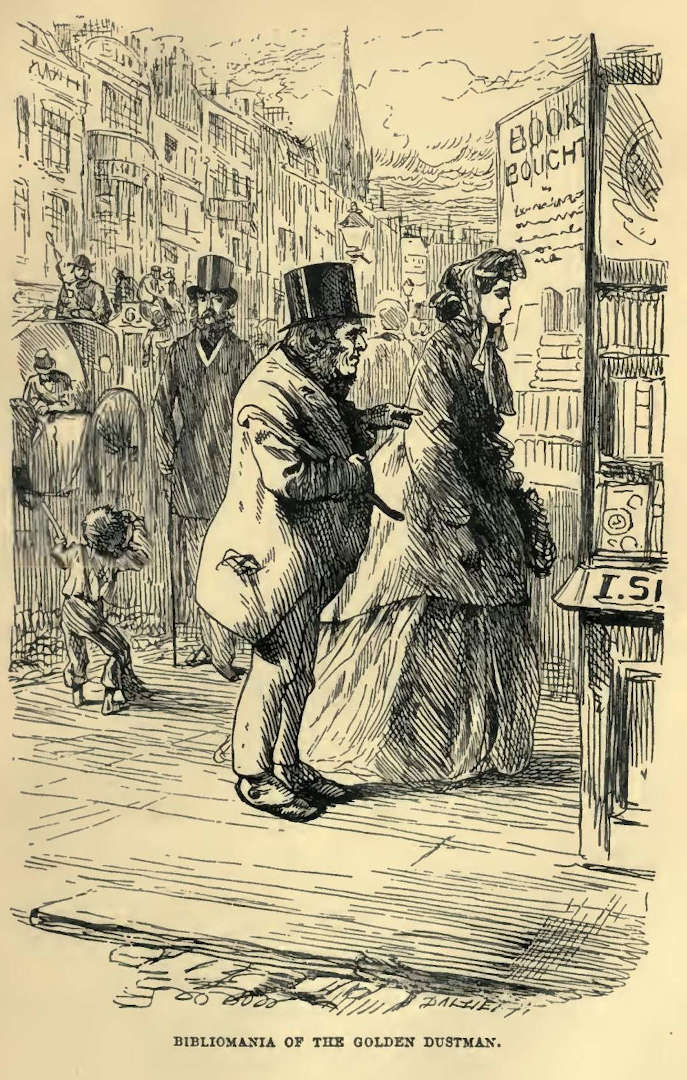
\includegraphics[scale=2.3]{03-05-01}

Chapter 14

CHECKMATE TO THE FRIENDLY MOVE


Mr and Mrs John Harmon had so timed their taking possession of their
rightful name and their London house, that the event befel on the very
day when the last waggon-load of the last Mound was driven out at the
gates of Boffin’s Bower. As it jolted away, Mr Wegg felt that the
last load was correspondingly removed from his mind, and hailed the
auspicious season when that black sheep, Boffin, was to be closely
sheared.

Over the whole slow process of levelling the Mounds, Silas had kept
watch with rapacious eyes. But, eyes no less rapacious had watched the
growth of the Mounds in years bygone, and had vigilantly sifted the dust
of which they were composed. No valuables turned up. How should there
be any, seeing that the old hard jailer of Harmony Jail had coined every
waif and stray into money, long before?

Though disappointed by this bare result, Mr Wegg felt too sensibly
relieved by the close of the labour, to grumble to any great extent.
A foreman-representative of the dust contractors, purchasers of the
Mounds, had worn Mr Wegg down to skin and bone. This supervisor of the
proceedings, asserting his employers’ rights to cart off by daylight,
nightlight, torchlight, when they would, must have been the death of
Silas if the work had lasted much longer. Seeming never to need sleep
himself, he would reappear, with a tied-up broken head, in fantail hat
and velveteen smalls, like an accursed goblin, at the most unholy and
untimely hours. Tired out by keeping close ward over a long day’s work
in fog and rain, Silas would have just crawled to bed and be dozing,
when a horrid shake and rumble under his pillow would announce an
approaching train of carts, escorted by this Demon of Unrest, to fall to
work again. At another time, he would be rumbled up out of his soundest
sleep, in the dead of the night; at another, would be kept at his post
eight-and-forty hours on end. The more his persecutor besought him not
to trouble himself to turn out, the more suspicious was the crafty Wegg
that indications had been observed of something hidden somewhere, and
that attempts were on foot to circumvent him. So continually broken was
his rest through these means, that he led the life of having wagered
to keep ten thousand dog-watches in ten thousand hours, and looked
piteously upon himself as always getting up and yet never going to bed.
So gaunt and haggard had he grown at last, that his wooden leg showed
disproportionate, and presented a thriving appearance in contrast
with the rest of his plagued body, which might almost have been termed
chubby.

However, Wegg’s comfort was, that all his disagreeables were now over,
and that he was immediately coming into his property. Of late, the
grindstone did undoubtedly appear to have been whirling at his own nose
rather than Boffin’s, but Boffin’s nose was now to be sharpened fine.
Thus far, Mr Wegg had let his dusty friend off lightly, having been
baulked in that amiable design of frequently dining with him, by the
machinations of the sleepless dustman. He had been constrained to depute
Mr Venus to keep their dusty friend, Boffin, under inspection, while he
himself turned lank and lean at the Bower.

To Mr Venus’s museum Mr Wegg repaired when at length the Mounds
were down and gone. It being evening, he found that gentleman, as he
expected, seated over his fire; but did not find him, as he expected,
floating his powerful mind in tea.

‘Why, you smell rather comfortable here!’ said Wegg, seeming to take it
ill, and stopping and sniffing as he entered.

‘I AM rather comfortable, sir,’ said Venus.

‘You don’t use lemon in your business, do you?’ asked Wegg, sniffing
again.

‘No, Mr Wegg,’ said Venus. ‘When I use it at all, I mostly use it in
cobblers’ punch.’

‘What do you call cobblers’ punch?’ demanded Wegg, in a worse humour
than before.

‘It’s difficult to impart the receipt for it, sir,’ returned Venus,
‘because, however particular you may be in allotting your materials,
so much will still depend upon the individual gifts, and there being a
feeling thrown into it. But the groundwork is gin.’

‘In a Dutch bottle?’ said Wegg gloomily, as he sat himself down.

‘Very good, sir, very good!’ cried Venus. ‘Will you partake, sir?’

‘Will I partake?’ returned Wegg very surlily. ‘Why, of course I will!
WILL a man partake, as has been tormented out of his five senses by
an everlasting dustman with his head tied up! WILL he, too! As if he
wouldn’t!’

‘Don’t let it put you out, Mr Wegg. You don’t seem in your usual
spirits.’

‘If you come to that, you don’t seem in your usual spirits,’ growled
Wegg. ‘You seem to be setting up for lively.’

This circumstance appeared, in his then state of mind, to give Mr Wegg
uncommon offence.

‘And you’ve been having your hair cut!’ said Wegg, missing the usual
dusty shock.

‘Yes, Mr Wegg. But don’t let that put you out, either.’

‘And I am blest if you ain’t getting fat!’ said Wegg, with culminating
discontent. ‘What are you going to do next?’

‘Well, Mr Wegg,’ said Venus, smiling in a sprightly manner, ‘I suspect
you could hardly guess what I am going to do next.’

‘I don’t want to guess,’ retorted Wegg. ‘All I’ve got to say is, that
it’s well for you that the diwision of labour has been what it has been.
It’s well for you to have had so light a part in this business, when
mine has been so heavy. You haven’t had YOUR rest broke, I’ll be bound.’

‘Not at all, sir,’ said Venus. ‘Never rested so well in all my life, I
thank you.’

‘Ah!’ grumbled Wegg, ‘you should have been me. If you had been me, and
had been fretted out of your bed, and your sleep, and your meals, and
your mind, for a stretch of months together, you’d have been out of
condition and out of sorts.’

‘Certainly, it has trained you down, Mr Wegg,’ said Venus, contemplating
his figure with an artist’s eye. ‘Trained you down very low, it has! So
weazen and yellow is the kivering upon your bones, that one might almost
fancy you had come to give a look-in upon the French gentleman in the
corner, instead of me.’

Mr Wegg, glancing in great dudgeon towards the French gentleman’s
corner, seemed to notice something new there, which induced him to
glance at the opposite corner, and then to put on his glasses and stare
at all the nooks and corners of the dim shop in succession.

‘Why, you’ve been having the place cleaned up!’ he exclaimed.

‘Yes, Mr Wegg. By the hand of adorable woman.’

‘Then what you’re going to do next, I suppose, is to get married?’

‘That’s it, sir.’

Silas took off his glasses again--finding himself too intensely
disgusted by the sprightly appearance of his friend and partner to bear
a magnified view of him and made the inquiry:

‘To the old party?’

‘Mr Wegg!’ said Venus, with a sudden flush of wrath. ‘The lady in
question is not a old party.’

‘I meant,’ exclaimed Wegg, testily, ‘to the party as formerly objected?’

‘Mr Wegg,’ said Venus, ‘in a case of so much delicacy, I must trouble
you to say what you mean. There are strings that must not be played
upon. No sir! Not sounded, unless in the most respectful and tuneful
manner. Of such melodious strings is Miss Pleasant Riderhood formed.’

‘Then it IS the lady as formerly objected?’ said Wegg.

‘Sir,’ returned Venus with dignity, ‘I accept the altered phrase. It is
the lady as formerly objected.’

‘When is it to come off?’ asked Silas.

‘Mr Wegg,’ said Venus, with another flush. ‘I cannot permit it to be
put in the form of a Fight. I must temperately but firmly call upon you,
sir, to amend that question.’

‘When is the lady,’ Wegg reluctantly demanded, constraining his ill
temper in remembrance of the partnership and its stock in trade, ‘a
going to give her ‘and where she has already given her ‘art?’

‘Sir,’ returned Venus, ‘I again accept the altered phrase, and with
pleasure. The lady is a going to give her ‘and where she has already
given her ‘art, next Monday.’

‘Then the lady’s objection has been met?’ said Silas.

‘Mr Wegg,’ said Venus, ‘as I did name to you, I think, on a former
occasion, if not on former occasions--’

‘On former occasions,’ interrupted Wegg.

‘--What,’ pursued Venus, ‘what the nature of the lady’s objection was, I
may impart, without violating any of the tender confidences since sprung
up between the lady and myself, how it has been met, through the kind
interference of two good friends of mine: one, previously acquainted
with the lady: and one, not. The pint was thrown out, sir, by those two
friends when they did me the great service of waiting on the lady to
try if a union betwixt the lady and me could not be brought to bear--the
pint, I say, was thrown out by them, sir, whether if, after marriage,
I confined myself to the articulation of men, children, and the lower
animals, it might not relieve the lady’s mind of her feeling respecting
being as a lady--regarded in a bony light. It was a happy thought, sir,
and it took root.’

‘It would seem, Mr Venus,’ observed Wegg, with a touch of distrust,
‘that you are flush of friends?’

‘Pretty well, sir,’ that gentleman answered, in a tone of placid
mystery. ‘So-so, sir. Pretty well.’

‘However,’ said Wegg, after eyeing him with another touch of distrust,
‘I wish you joy. One man spends his fortune in one way, and another in
another. You are going to try matrimony. I mean to try travelling.’

‘Indeed, Mr Wegg?’

‘Change of air, sea-scenery, and my natural rest, I hope may bring me
round after the persecutions I have undergone from the dustman with his
head tied up, which I just now mentioned. The tough job being ended and
the Mounds laid low, the hour is come for Boffin to stump up. Would ten
to-morrow morning suit you, partner, for finally bringing Boffin’s nose
to the grindstone?’

Ten to-morrow morning would quite suit Mr Venus for that excellent
purpose.

‘You have had him well under inspection, I hope?’ said Silas.

Mr Venus had had him under inspection pretty well every day.

‘Suppose you was just to step round to-night then, and give him orders
from me--I say from me, because he knows I won’t be played with--to be
ready with his papers, his accounts, and his cash, at that time in the
morning?’ said Wegg. ‘And as a matter of form, which will be agreeable
to your own feelings, before we go out (for I’ll walk with you part of
the way, though my leg gives under me with weariness), let’s have a look
at the stock in trade.’

Mr Venus produced it, and it was perfectly correct; Mr Venus undertook
to produce it again in the morning, and to keep tryst with Mr Wegg on
Boffin’s doorstep as the clock struck ten. At a certain point of the
road between Clerkenwell and Boffin’s house (Mr Wegg expressly insisted
that there should be no prefix to the Golden Dustman’s name) the
partners separated for the night.

It was a very bad night; to which succeeded a very bad morning. The
streets were so unusually slushy, muddy, and miserable, in the morning,
that Wegg rode to the scene of action; arguing that a man who was, as
it were, going to the Bank to draw out a handsome property, could well
afford that trifling expense.

Venus was punctual, and Wegg undertook to knock at the door, and conduct
the conference. Door knocked at. Door opened.

‘Boffin at home?’

The servant replied that MR Boffin was at home.

‘He’ll do,’ said Wegg, ‘though it ain’t what I call him.’

The servant inquired if they had any appointment?

‘Now, I tell you what, young fellow,’ said Wegg, ‘I won’t have it. This
won’t do for me. I don’t want menials. I want Boffin.’

They were shown into a waiting-room, where the all-powerful Wegg wore
his hat, and whistled, and with his forefinger stirred up a clock that
stood upon the chimneypiece, until he made it strike. In a few minutes
they were shown upstairs into what used to be Boffin’s room; which,
besides the door of entrance, had folding-doors in it, to make it one
of a suite of rooms when occasion required. Here, Boffin was seated at a
library-table, and here Mr Wegg, having imperiously motioned the servant
to withdraw, drew up a chair and seated himself, in his hat, close
beside him. Here, also, Mr Wegg instantly underwent the remarkable
experience of having his hat twitched off his head and thrown out of a
window, which was opened and shut for the purpose.

‘Be careful what insolent liberties you take in that gentleman’s
presence,’ said the owner of the hand which had done this, ‘or I will
throw you after it.’

Wegg involuntarily clapped his hand to his bare head, and stared at the
Secretary. For, it was he addressed him with a severe countenance, and
who had come in quietly by the folding-doors.

‘Oh!’ said Wegg, as soon as he recovered his suspended power of speech.
‘Very good! I gave directions for YOU to be dismissed. And you ain’t
gone, ain’t you? Oh! We’ll look into this presently. Very good!’

‘No, nor I ain’t gone,’ said another voice.

Somebody else had come in quietly by the folding-doors. Turning his
head, Wegg beheld his persecutor, the ever-wakeful dustman, accoutred
with fantail hat and velveteen smalls complete. Who, untying his
tied-up broken head, revealed a head that was whole, and a face that was
Sloppy’s.

‘Ha, ha, ha, gentlemen!’ roared Sloppy in a peal of laughter, and with
immeasureable relish. ‘He never thought as I could sleep standing, and
often done it when I turned for Mrs Higden! He never thought as I used
to give Mrs Higden the Police-news in different voices! But I did lead
him a life all through it, gentlemen, I hope I really and truly DID!’
Here, Mr Sloppy opening his mouth to a quite alarming extent, and
throwing back his head to peal again, revealed incalculable buttons.

‘Oh!’ said Wegg, slightly discomfited, but not much as yet: ‘one and one
is two not dismissed, is it? Bof--fin! Just let me ask a question. Who
set this chap on, in this dress, when the carting began? Who employed
this fellow?’

‘I say!’ remonstrated Sloppy, jerking his head forward. ‘No fellows, or
I’ll throw you out of winder!’

Mr Boffin appeased him with a wave of his hand, and said: ‘I employed
him, Wegg.’

‘Oh! You employed him, Boffin? Very good. Mr Venus, we raise our terms,
and we can’t do better than proceed to business. Bof--fin! I want the
room cleared of these two scum.’

‘That’s not going to be done, Wegg,’ replied Mr Boffin, sitting
composedly on the library-table, at one end, while the Secretary sat
composedly on it at the other.

‘Bof--fin! Not going to be done?’ repeated Wegg. ‘Not at your peril?’

‘No, Wegg,’ said Mr Boffin, shaking his head good-humouredly. ‘Not at my
peril, and not on any other terms.’

Wegg reflected a moment, and then said: ‘Mr Venus, will you be so good
as hand me over that same dockyment?’

‘Certainly, sir,’ replied Venus, handing it to him with much politeness.
‘There it is. Having now, sir, parted with it, I wish to make a small
observation: not so much because it is anyways necessary, or expresses
any new doctrine or discovery, as because it is a comfort to my mind.
Silas Wegg, you are a precious old rascal.’

Mr Wegg, who, as if anticipating a compliment, had been beating
time with the paper to the other’s politeness until this unexpected
conclusion came upon him, stopped rather abruptly.

‘Silas Wegg,’ said Venus, ‘know that I took the liberty of taking Mr
Boffin into our concern as a sleeping partner, at a very early period of
our firm’s existence.’

‘Quite true,’ added Mr Boffin; ‘and I tested Venus by making him a
pretended proposal or two; and I found him on the whole a very honest
man, Wegg.’

‘So Mr Boffin, in his indulgence, is pleased to say,’ Venus remarked:
‘though in the beginning of this dirt, my hands were not, for a few
hours, quite as clean as I could wish. But I hope I made early and full
amends.’

‘Venus, you did,’ said Mr Boffin. ‘Certainly, certainly, certainly.’

Venus inclined his head with respect and gratitude. ‘Thank you, sir.
I am much obliged to you, sir, for all. For your good opinion now, for
your way of receiving and encouraging me when I first put myself in
communication with you, and for the influence since so kindly brought
to bear upon a certain lady, both by yourself and by Mr John Harmon.’ To
whom, when thus making mention of him, he also bowed.

Wegg followed the name with sharp ears, and the action with sharp eyes,
and a certain cringing air was infusing itself into his bullying air,
when his attention was re-claimed by Venus.

‘Everything else between you and me, Mr Wegg,’ said Venus, ‘now explains
itself, and you can now make out, sir, without further words from me.
But totally to prevent any unpleasantness or mistake that might arise on
what I consider an important point, to be made quite clear at the close
of our acquaintance, I beg the leave of Mr Boffin and Mr John Harmon to
repeat an observation which I have already had the pleasure of bringing
under your notice. You are a precious old rascal!’

‘You are a fool,’ said Wegg, with a snap of his fingers, ‘and I’d have
got rid of you before now, if I could have struck out any way of doing
it. I have thought it over, I can tell you. You may go, and welcome. You
leave the more for me. Because, you know,’ said Wegg, dividing his next
observation between Mr Boffin and Mr Harmon, ‘I am worth my price, and
I mean to have it. This getting off is all very well in its way, and it
tells with such an anatomical Pump as this one,’ pointing out Mr Venus,
‘but it won’t do with a Man. I am here to be bought off, and I have
named my figure. Now, buy me, or leave me.’

‘I’ll leave you, Wegg,’ said Mr Boffin, laughing, ‘as far as I am
concerned.’

‘Bof--fin!’ replied Wegg, turning upon him with a severe air, ‘I
understand YOUR new-born boldness. I see the brass underneath YOUR
silver plating. YOU have got YOUR nose out of joint. Knowing that you’ve
nothing at stake, you can afford to come the independent game. Why,
you’re just so much smeary glass to see through, you know! But Mr Harmon
is in another sitiwation. What Mr Harmon risks, is quite another pair
of shoes. Now, I’ve heerd something lately about this being Mr
Harmon--I make out now, some hints that I’ve met on that subject in
the newspaper--and I drop you, Bof--fin, as beneath my notice. I ask Mr
Harmon whether he has any idea of the contents of this present paper?’

‘It is a will of my late father’s, of more recent date than the will
proved by Mr Boffin (address whom again, as you have addressed him
already, and I’ll knock you down), leaving the whole of his property
to the Crown,’ said John Harmon, with as much indifference as was
compatible with extreme sternness.

‘Bight you are!’ cried Wegg. ‘Then,’ screwing the weight of his body
upon his wooden leg, and screwing his wooden head very much on one side,
and screwing up one eye: ‘then, I put the question to you, what’s this
paper worth?’

‘Nothing,’ said John Harmon.

Wegg had repeated the word with a sneer, and was entering on some
sarcastic retort, when, to his boundless amazement, he found himself
gripped by the cravat; shaken until his teeth chattered; shoved back,
staggering, into a corner of the room; and pinned there.

‘You scoundrel!’ said John Harmon, whose seafaring hold was like that of
a vice.

‘You’re knocking my head against the wall,’ urged Silas faintly.

‘I mean to knock your head against the wall,’ returned John Harmon,
suiting his action to his words, with the heartiest good will; ‘and I’d
give a thousand pounds for leave to knock your brains out. Listen, you
scoundrel, and look at that Dutch bottle.’

Sloppy held it up, for his edification.

‘That Dutch bottle, scoundrel, contained the latest will of the many
wills made by my unhappy self-tormenting father. That will gives
everything absolutely to my noble benefactor and yours, Mr Boffin,
excluding and reviling me, and my sister (then already dead of a broken
heart), by name. That Dutch bottle was found by my noble benefactor and
yours, after he entered on possession of the estate. That Dutch bottle
distressed him beyond measure, because, though I and my sister were
both no more, it cast a slur upon our memory which he knew we had
done nothing in our miserable youth, to deserve. That Dutch bottle,
therefore, he buried in the Mound belonging to him, and there it lay
while you, you thankless wretch, were prodding and poking--often very
near it, I dare say. His intention was, that it should never see the
light; but he was afraid to destroy it, lest to destroy such a document,
even with his great generous motive, might be an offence at law. After
the discovery was made here who I was, Mr Boffin, still restless on the
subject, told me, upon certain conditions impossible for such a hound as
you to appreciate, the secret of that Dutch bottle. I urged upon him the
necessity of its being dug up, and the paper being legally produced and
established. The first thing you saw him do, and the second thing has
been done without your knowledge. Consequently, the paper now rattling
in your hand as I shake you--and I should like to shake the life out
of you--is worth less than the rotten cork of the Dutch bottle, do you
understand?’

Judging from the fallen countenance of Silas as his head wagged
backwards and forwards in a most uncomfortable manner, he did
understand.

‘Now, scoundrel,’ said John Harmon, taking another sailor-like turn on
his cravat and holding him in his corner at arms’ length, ‘I shall make
two more short speeches to you, because I hope they will torment you.
Your discovery was a genuine discovery (such as it was), for nobody had
thought of looking into that place. Neither did we know you had made it,
until Venus spoke to Mr Boffin, though I kept you under good observation
from my first appearance here, and though Sloppy has long made it
the chief occupation and delight of his life, to attend you like your
shadow. I tell you this, that you may know we knew enough of you to
persuade Mr Boffin to let us lead you on, deluded, to the last possible
moment, in order that your disappointment might be the heaviest possible
disappointment. That’s the first short speech, do you understand?’

Here, John Harmon assisted his comprehension with another shake.

‘Now, scoundrel,’ he pursued, ‘I am going to finish. You supposed me
just now, to be the possessor of my father’s property.--So I am. But
through any act of my father’s, or by any right I have? No. Through the
munificence of Mr Boffin. The conditions that he made with me, before
parting with the secret of the Dutch bottle, were, that I should take
the fortune, and that he should take his Mound and no more. I owe
everything I possess, solely to the disinterestedness, uprightness,
tenderness, goodness (there are no words to satisfy me) of Mr and Mrs
Boffin. And when, knowing what I knew, I saw such a mud-worm as you
presume to rise in this house against this noble soul, the wonder is,’
added John Harmon through his clenched teeth, and with a very ugly turn
indeed on Wegg’s cravat, ‘that I didn’t try to twist your head off,
and fling THAT out of window! So. That’s the last short speech, do you
understand?’

Silas, released, put his hand to his throat, cleared it, and looked as
if he had a rather large fishbone in that region. Simultaneously with
this action on his part in his corner, a singular, and on the surface
an incomprehensible, movement was made by Mr Sloppy: who began backing
towards Mr Wegg along the wall, in the manner of a porter or heaver who
is about to lift a sack of flour or coals.

‘I am sorry, Wegg,’ said Mr Boffin, in his clemency, ‘that my old lady
and I can’t have a better opinion of you than the bad one we are forced
to entertain. But I shouldn’t like to leave you, after all said and
done, worse off in life than I found you. Therefore say in a word,
before we part, what it’ll cost to set you up in another stall.’

‘And in another place,’ John Harmon struck in. ‘You don’t come outside
these windows.’

‘Mr Boffin,’ returned Wegg in avaricious humiliation: ‘when I first had
the honour of making your acquaintance, I had got together a collection
of ballads which was, I may say, above price.’

‘Then they can’t be paid for,’ said John Harmon, ‘and you had better not
try, my dear sir.’

‘Pardon me, Mr Boffin,’ resumed Wegg, with a malignant glance in the
last speaker’s direction, ‘I was putting the case to you, who, if my
senses did not deceive me, put the case to me. I had a very choice
collection of ballads, and there was a new stock of gingerbread in the
tin box. I say no more, but would rather leave it to you.’

‘But it’s difficult to name what’s right,’ said Mr Boffin uneasily, with
his hand in his pocket, ‘and I don’t want to go beyond what’s right,
because you really have turned out such a very bad fellow. So artful,
and so ungrateful you have been, Wegg; for when did I ever injure you?’

‘There was also,’ Mr Wegg went on, in a meditative manner, ‘a errand
connection, in which I was much respected. But I would not wish to be
deemed covetous, and I would rather leave it to you, Mr Boffin.’

‘Upon my word, I don’t know what to put it at,’ the Golden Dustman
muttered.

‘There was likewise,’ resumed Wegg, ‘a pair of trestles, for which alone
a Irish person, who was deemed a judge of trestles, offered five and
six--a sum I would not hear of, for I should have lost by it--and there
was a stool, a umbrella, a clothes-horse, and a tray. But I leave it to
you, Mr Boffin.’

The Golden Dustman seeming to be engaged in some abstruse calculation,
Mr Wegg assisted him with the following additional items.

‘There was, further, Miss Elizabeth, Master George, Aunt Jane, and Uncle
Parker. Ah! When a man thinks of the loss of such patronage as that;
when a man finds so fair a garden rooted up by pigs; he finds it hard
indeed, without going high, to work it into money. But I leave it wholly
to you, sir.’

Mr Sloppy still continued his singular, and on the surface his
incomprehensible, movement.

‘Leading on has been mentioned,’ said Wegg with a melancholy air, ‘and
it’s not easy to say how far the tone of my mind may have been lowered
by unwholesome reading on the subject of Misers, when you was leading me
and others on to think you one yourself, sir. All I can say is, that
I felt my tone of mind a lowering at the time. And how can a man put a
price upon his mind! There was likewise a hat just now. But I leave the
ole to you, Mr Boffin.’

‘Come!’ said Mr Boffin. ‘Here’s a couple of pound.’

‘In justice to myself, I couldn’t take it, sir.’

The words were but out of his mouth when John Harmon lifted his finger,
and Sloppy, who was now close to Wegg, backed to Wegg’s back, stooped,
grasped his coat collar behind with both hands, and deftly swung him
up like the sack of flour or coals before mentioned. A countenance of
special discontent and amazement Mr Wegg exhibited in this position,
with his buttons almost as prominently on view as Sloppy’s own, and
with his wooden leg in a highly unaccommodating state. But, not for many
seconds was his countenance visible in the room; for, Sloppy lightly
trotted out with him and trotted down the staircase, Mr Venus attending
to open the street door. Mr Sloppy’s instructions had been to deposit
his burden in the road; but, a scavenger’s cart happening to stand
unattended at the corner, with its little ladder planted against the
wheel, Mr S. found it impossible to resist the temptation of shooting Mr
Silas Wegg into the cart’s contents. A somewhat difficult feat, achieved
with great dexterity, and with a prodigious splash.



Chapter 15

WHAT WAS CAUGHT IN THE TRAPS THAT WERE SET


How Bradley Headstone had been racked and riven in his mind since the
quiet evening when by the river-side he had risen, as it were, out of
the ashes of the Bargeman, none but he could have told. Not even he
could have told, for such misery can only be felt.

First, he had to bear the combined weight of the knowledge of what he
had done, of that haunting reproach that he might have done it so much
better, and of the dread of discovery. This was load enough to crush
him, and he laboured under it day and night. It was as heavy on him in
his scanty sleep, as in his red-eyed waking hours. It bore him down with
a dread unchanging monotony, in which there was not a moment’s variety.
The overweighted beast of burden, or the overweighted slave, can for
certain instants shift the physical load, and find some slight respite
even in enforcing additional pain upon such a set of muscles or such
a limb. Not even that poor mockery of relief could the wretched man
obtain, under the steady pressure of the infernal atmosphere into which
he had entered.

Time went by, and no visible suspicion dogged him; time went by, and
in such public accounts of the attack as were renewed at intervals,
he began to see Mr Lightwood (who acted as lawyer for the injured man)
straying further from the fact, going wider of the issue, and evidently
slackening in his zeal. By degrees, a glimmering of the cause of this
began to break on Bradley’s sight. Then came the chance meeting with Mr
Milvey at the railway station (where he often lingered in his leisure
hours, as a place where any fresh news of his deed would be circulated,
or any placard referring to it would be posted), and then he saw in the
light what he had brought about.

For, then he saw that through his desperate attempt to separate those
two for ever, he had been made the means of uniting them. That he had
dipped his hands in blood, to mark himself a miserable fool and tool.
That Eugene Wrayburn, for his wife’s sake, set him aside and left him to
crawl along his blasted course. He thought of Fate, or Providence, or
be the directing Power what it might, as having put a fraud upon
him--overreached him--and in his impotent mad rage bit, and tore, and
had his fit.

New assurance of the truth came upon him in the next few following days,
when it was put forth how the wounded man had been married on his bed,
and to whom, and how, though always in a dangerous condition, he was a
shade better. Bradley would far rather have been seized for his murder,
than he would have read that passage, knowing himself spared, and
knowing why.

But, not to be still further defrauded and overreached--which he would
be, if implicated by Riderhood, and punished by the law for his abject
failure, as though it had been a success--he kept close in his school
during the day, ventured out warily at night, and went no more to the
railway station. He examined the advertisements in the newspapers for
any sign that Riderhood acted on his hinted threat of so summoning him
to renew their acquaintance, but found none. Having paid him handsomely
for the support and accommodation he had had at the Lock House, and
knowing him to be a very ignorant man who could not write, he began to
doubt whether he was to be feared at all, or whether they need ever meet
again.

All this time, his mind was never off the rack, and his raging sense of
having been made to fling himself across the chasm which divided those
two, and bridge it over for their coming together, never cooled down.
This horrible condition brought on other fits. He could not have said
how many, or when; but he saw in the faces of his pupils that they had
seen him in that state, and that they were possessed by a dread of his
relapsing.

One winter day when a slight fall of snow was feathering the sills and
frames of the schoolroom windows, he stood at his black board, crayon in
hand, about to commence with a class; when, reading in the countenances
of those boys that there was something wrong, and that they seemed in
alarm for him, he turned his eyes to the door towards which they faced.
He then saw a slouching man of forbidding appearance standing in the
midst of the school, with a bundle under his arm; and saw that it was
Riderhood.

He sat down on a stool which one of his boys put for him, and he had a
passing knowledge that he was in danger of falling, and that his face
was becoming distorted. But, the fit went off for that time, and he
wiped his mouth, and stood up again.

‘Beg your pardon, governor! By your leave!’ said Riderhood, knuckling
his forehead, with a chuckle and a leer. ‘What place may this be?’

‘This is a school.’

‘Where young folks learns wot’s right?’ said Riderhood, gravely nodding.
‘Beg your pardon, governor! By your leave! But who teaches this school?’

‘I do.’

‘You’re the master, are you, learned governor?’

‘Yes. I am the master.’

‘And a lovely thing it must be,’ said Riderhood, ‘fur to learn young
folks wot’s right, and fur to know wot THEY know wot you do it. Beg your
pardon, learned governor! By your leave!--That there black board; wot’s
it for?’

‘It is for drawing on, or writing on.’

‘Is it though!’ said Riderhood. ‘Who’d have thought it, from the
looks on it! WOULD you be so kind as write your name upon it, learned
governor?’ (In a wheedling tone.)

Bradley hesitated for a moment; but placed his usual signature,
enlarged, upon the board.

‘I ain’t a learned character myself,’ said Riderhood, surveying the
class, ‘but I do admire learning in others. I should dearly like to hear
these here young folks read that there name off, from the writing.’

The arms of the class went up. At the miserable master’s nod, the shrill
chorus arose: ‘Bradley Headstone!’

‘No?’ cried Riderhood. ‘You don’t mean it? Headstone! Why, that’s in a
churchyard. Hooroar for another turn!’

Another tossing of arms, another nod, and another shrill chorus:

‘Bradley Headstone!’

‘I’ve got it now!’ said Riderhood, after attentively listening, and
internally repeating: ‘Bradley. I see. Chris’en name, Bradley sim’lar to
Roger which is my own. Eh? Fam’ly name, Headstone, sim’lar to Riderhood
which is my own. Eh?’

Shrill chorus. ‘Yes!’

‘Might you be acquainted, learned governor,’ said Riderhood, ‘with a
person of about your own heighth and breadth, and wot ‘ud pull down in
a scale about your own weight, answering to a name sounding summat like
Totherest?’

With a desperation in him that made him perfectly quiet, though his jaw
was heavily squared; with his eyes upon Riderhood; and with traces of
quickened breathing in his nostrils; the schoolmaster replied, in a
suppressed voice, after a pause: ‘I think I know the man you mean.’

‘I thought you knowed the man I mean, learned governor. I want the man.’

With a half glance around him at his pupils, Bradley returned:

‘Do you suppose he is here?’

‘Begging your pardon, learned governor, and by your leave,’ said
Riderhood, with a laugh, ‘how could I suppose he’s here, when there’s
nobody here but you, and me, and these young lambs wot you’re a learning
on? But he is most excellent company, that man, and I want him to come
and see me at my Lock, up the river.’

‘I’ll tell him so.’

‘D’ye think he’ll come?’ asked Riderhood.

‘I am sure he will.’

‘Having got your word for him,’ said Riderhood, ‘I shall count upon him.
P’raps you’d so fur obleege me, learned governor, as tell him that if he
don’t come precious soon, I’ll look him up.’

‘He shall know it.’

‘Thankee. As I says a while ago,’ pursued Riderhood, changing his hoarse
tone and leering round upon the class again, ‘though not a learned
character my own self, I do admire learning in others, to be sure! Being
here and having met with your kind attention, Master, might I, afore I
go, ask a question of these here young lambs of yourn?’

‘If it is in the way of school,’ said Bradley, always sustaining his
dark look at the other, and speaking in his suppressed voice, ‘you may.’

‘Oh! It’s in the way of school!’ cried Riderhood. ‘I’ll pound it,
Master, to be in the way of school. Wot’s the diwisions of water, my
lambs? Wot sorts of water is there on the land?’

Shrill chorus: ‘Seas, rivers, lakes, and ponds.’

‘Seas, rivers, lakes, and ponds,’ said Riderhood. ‘They’ve got all the
lot, Master! Blowed if I shouldn’t have left out lakes, never having
clapped eyes upon one, to my knowledge. Seas, rivers, lakes, and ponds.
Wot is it, lambs, as they ketches in seas, rivers, lakes, and ponds?’

Shrill chorus (with some contempt for the ease of the question):

‘Fish!’

‘Good a-gin!’ said Riderhood. ‘But wot else is it, my lambs, as they
sometimes ketches in rivers?’

Chorus at a loss. One shrill voice: ‘Weed!’

‘Good agin!’ cried Riderhood. ‘But it ain’t weed neither. You’ll never
guess, my dears. Wot is it, besides fish, as they sometimes ketches in
rivers? Well! I’ll tell you. It’s suits o’ clothes.’

Bradley’s face changed.

‘Leastways, lambs,’ said Riderhood, observing him out of the corners
of his eyes, ‘that’s wot I my own self sometimes ketches in rivers. For
strike me blind, my lambs, if I didn’t ketch in a river the wery bundle
under my arm!’

The class looked at the master, as if appealing from the irregular
entrapment of this mode of examination. The master looked at the
examiner, as if he would have torn him to pieces.

‘I ask your pardon, learned governor,’ said Riderhood, smearing his
sleeve across his mouth as he laughed with a relish, ‘tain’t fair to the
lambs, I know. It wos a bit of fun of mine. But upon my soul I drawed
this here bundle out of a river! It’s a Bargeman’s suit of clothes. You
see, it had been sunk there by the man as wore it, and I got it up.’

‘How do you know it was sunk by the man who wore it?’ asked Bradley.

‘Cause I see him do it,’ said Riderhood.

They looked at each other. Bradley, slowly withdrawing his eyes, turned
his face to the black board and slowly wiped his name out.

‘A heap of thanks, Master,’ said Riderhood, ‘for bestowing so much of
your time, and of the lambses’ time, upon a man as hasn’t got no other
recommendation to you than being a honest man. Wishing to see at my Lock
up the river, the person as we’ve spoke of, and as you’ve answered for,
I takes my leave of the lambs and of their learned governor both.’

With those words, he slouched out of the school, leaving the master
to get through his weary work as he might, and leaving the whispering
pupils to observe the master’s face until he fell into the fit which had
been long impending.

The next day but one was Saturday, and a holiday. Bradley rose early,
and set out on foot for Plashwater Weir Mill Lock. He rose so early that
it was not yet light when he began his journey. Before extinguishing the
candle by which he had dressed himself, he made a little parcel of his
decent silver watch and its decent guard, and wrote inside the paper:
‘Kindly take care of these for me.’ He then addressed the parcel to Miss
Peecher, and left it on the most protected corner of the little seat in
her little porch.

It was a cold hard easterly morning when he latched the garden gate
and turned away. The light snowfall which had feathered his schoolroom
windows on the Thursday, still lingered in the air, and was falling
white, while the wind blew black. The tardy day did not appear until he
had been on foot two hours, and had traversed a greater part of London
from east to west. Such breakfast as he had, he took at the comfortless
public-house where he had parted from Riderhood on the occasion of
their night-walk. He took it, standing at the littered bar, and looked
loweringly at a man who stood where Riderhood had stood that early
morning.

He outwalked the short day, and was on the towing-path by the river,
somewhat footsore, when the night closed in. Still two or three miles
short of the Lock, he slackened his pace then, but went steadily on. The
ground was now covered with snow, though thinly, and there were floating
lumps of ice in the more exposed parts of the river, and broken sheets
of ice under the shelter of the banks. He took heed of nothing but the
ice, the snow, and the distance, until he saw a light ahead, which he
knew gleamed from the Lock House window. It arrested his steps, and he
looked all around. The ice, and the snow, and he, and the one light, had
absolute possession of the dreary scene. In the distance before him, lay
the place where he had struck the worse than useless blows that mocked
him with Lizzie’s presence there as Eugene’s wife. In the distance
behind him, lay the place where the children with pointing arms had
seemed to devote him to the demons in crying out his name. Within there,
where the light was, was the man who as to both distances could give him
up to ruin. To these limits had his world shrunk.

He mended his pace, keeping his eyes upon the light with a strange
intensity, as if he were taking aim at it. When he approached it so
nearly as that it parted into rays, they seemed to fasten themselves
to him and draw him on. When he struck the door with his hand, his foot
followed so quickly on his hand, that he was in the room before he was
bidden to enter.

The light was the joint product of a fire and a candle. Between the two,
with his feet on the iron fender, sat Riderhood, pipe in mouth.

He looked up with a surly nod when his visitor came in. His visitor
looked down with a surly nod. His outer clothing removed, the visitor
then took a seat on the opposite side of the fire.

‘Not a smoker, I think?’ said Riderhood, pushing a bottle to him across
the table.

‘No.’

They both lapsed into silence, with their eyes upon the fire.

‘You don’t need to be told I am here,’ said Bradley at length. ‘Who is
to begin?’

‘I’ll begin,’ said Riderhood, ‘when I’ve smoked this here pipe out.’

He finished it with great deliberation, knocked out the ashes on the
hob, and put it by.

‘I’ll begin,’ he then repeated, ‘Bradley Headstone, Master, if you wish
it.’

‘Wish it? I wish to know what you want with me.’

‘And so you shall.’ Riderhood had looked hard at his hands and his
pockets, apparently as a precautionary measure lest he should have any
weapon about him. But, he now leaned forward, turning the collar of
his waistcoat with an inquisitive finger, and asked, ‘Why, where’s your
watch?’

‘I have left it behind.’

‘I want it. But it can be fetched. I’ve took a fancy to it.’

Bradley answered with a contemptuous laugh.

‘I want it,’ repeated Riderhood, in a louder voice, ‘and I mean to have
it.’

‘That is what you want of me, is it?’

‘No,’ said Riderhood, still louder; ‘it’s on’y part of what I want of
you. I want money of you.’

‘Anything else?’

‘Everythink else!’ roared Riderhood, in a very loud and furious way.
‘Answer me like that, and I won’t talk to you at all.’

Bradley looked at him.

‘Don’t so much as look at me like that, or I won’t talk to you at all,’
vociferated Riderhood. ‘But, instead of talking, I’ll bring my hand
down upon you with all its weight,’ heavily smiting the table with great
force, ‘and smash you!’

‘Go on,’ said Bradley, after moistening his lips.

‘O! I’m a going on. Don’t you fear but I’ll go on full-fast enough for
you, and fur enough for you, without your telling. Look here, Bradley
Headstone, Master. You might have split the T’other governor to chips
and wedges, without my caring, except that I might have come upon you
for a glass or so now and then. Else why have to do with you at all? But
when you copied my clothes, and when you copied my neckhankercher, and
when you shook blood upon me after you had done the trick, you did wot
I’ll be paid for and paid heavy for. If it come to be throw’d upon you,
you was to be ready to throw it upon me, was you? Where else but
in Plashwater Weir Mill Lock was there a man dressed according as
described? Where else but in Plashwater Weir Mill Lock was there a
man as had had words with him coming through in his boat? Look at the
Lock-keeper in Plashwater Weir Mill Lock, in them same answering clothes
and with that same answering red neckhankercher, and see whether his
clothes happens to be bloody or not. Yes, they do happen to be bloody.
Ah, you sly devil!’

Bradley, very white, sat looking at him in silence.

‘But two could play at your game,’ said Riderhood, snapping his fingers
at him half a dozen times, ‘and I played it long ago; long afore you
tried your clumsy hand at it; in days when you hadn’t begun croaking
your lecters or what not in your school. I know to a figure how you
done it. Where you stole away, I could steal away arter you, and do it
knowinger than you. I know how you come away from London in your own
clothes, and where you changed your clothes, and hid your clothes. I see
you with my own eyes take your own clothes from their hiding-place
among them felled trees, and take a dip in the river to account for
your dressing yourself, to any one as might come by. I see you rise up
Bradley Headstone, Master, where you sat down Bargeman. I see you pitch
your Bargeman’s bundle into the river. I hooked your Bargeman’s bundle
out of the river. I’ve got your Bargeman’s clothes, tore this way and
that way with the scuffle, stained green with the grass, and spattered
all over with what bust from the blows. I’ve got them, and I’ve got you.
I don’t care a curse for the T’other governor, alive or dead, but I care
a many curses for my own self. And as you laid your plots agin me and
was a sly devil agin me, I’ll be paid for it--I’ll be paid for it--I’ll
be paid for it--till I’ve drained you dry!’

Bradley looked at the fire, with a working face, and was silent for a
while. At last he said, with what seemed an inconsistent composure of
voice and feature:

‘You can’t get blood out of a stone, Riderhood.’

‘I can get money out of a schoolmaster though.’

‘You can’t get out of me what is not in me. You can’t wrest from me what
I have not got. Mine is but a poor calling. You have had more than two
guineas from me, already. Do you know how long it has taken me (allowing
for a long and arduous training) to earn such a sum?’

‘I don’t know, nor I don’t care. Yours is a ‘spectable calling. To
save your ‘spectability, it’s worth your while to pawn every article of
clothes you’ve got, sell every stick in your house, and beg and borrow
every penny you can get trusted with. When you’ve done that and handed
over, I’ll leave you. Not afore.’

‘How do you mean, you’ll leave me?’

‘I mean as I’ll keep you company, wherever you go, when you go away from
here. Let the Lock take care of itself. I’ll take care of you, once I’ve
got you.’

Bradley again looked at the fire. Eyeing him aside, Riderhood took up
his pipe, refilled it, lighted it, and sat smoking. Bradley leaned his
elbows on his knees, and his head upon his hands, and looked at the fire
with a most intent abstraction.

‘Riderhood,’ he said, raising himself in his chair, after a long
silence, and drawing out his purse and putting it on the table. ‘Say
I part with this, which is all the money I have; say I let you have
my watch; say that every quarter, when I draw my salary, I pay you a
certain portion of it.’

‘Say nothink of the sort,’ retorted Riderhood, shaking his head as he
smoked. ‘You’ve got away once, and I won’t run the chance agin. I’ve had
trouble enough to find you, and shouldn’t have found you, if I hadn’t
seen you slipping along the street overnight, and watched you till you
was safe housed. I’ll have one settlement with you for good and all.’

‘Riderhood, I am a man who has lived a retired life. I have no resources
beyond myself. I have absolutely no friends.’

‘That’s a lie,’ said Riderhood. ‘You’ve got one friend as I knows of;
one as is good for a Savings-Bank book, or I’m a blue monkey!’

Bradley’s face darkened, and his hand slowly closed on the purse and
drew it back, as he sat listening for what the other should go on to
say.

‘I went into the wrong shop, fust, last Thursday,’ said Riderhood.
‘Found myself among the young ladies, by George! Over the young ladies,
I see a Missis. That Missis is sweet enough upon you, Master, to sell
herself up, slap, to get you out of trouble. Make her do it then.’

Bradley stared at him so very suddenly that Riderhood, not quite knowing
how to take it, affected to be occupied with the encircling smoke from
his pipe; fanning it away with his hand, and blowing it off.

‘You spoke to the mistress, did you?’ inquired Bradley, with that
former composure of voice and feature that seemed inconsistent, and with
averted eyes.

‘Poof! Yes,’ said Riderhood, withdrawing his attention from the smoke.
‘I spoke to her. I didn’t say much to her. She was put in a fluster by
my dropping in among the young ladies (I never did set up for a lady’s
man), and she took me into her parlour to hope as there was nothink
wrong. I tells her, “O no, nothink wrong. The master’s my wery good
friend.” But I see how the land laid, and that she was comfortable off.’

Bradley put the purse in his pocket, grasped his left wrist with his
right hand, and sat rigidly contemplating the fire.

‘She couldn’t live more handy to you than she does,’ said Riderhood,
‘and when I goes home with you (as of course I am a going), I recommend
you to clean her out without loss of time. You can marry her, arter you
and me have come to a settlement. She’s nice-looking, and I know
you can’t be keeping company with no one else, having been so lately
disapinted in another quarter.’

Not one other word did Bradley utter all that night. Not once did he
change his attitude, or loosen his hold upon his wrist. Rigid before the
fire, as if it were a charmed flame that was turning him old, he sat,
with the dark lines deepening in his face, its stare becoming more and
more haggard, its surface turning whiter and whiter as if it were being
overspread with ashes, and the very texture and colour of his hair
degenerating.

Not until the late daylight made the window transparent, did this
decaying statue move. Then it slowly arose, and sat in the window
looking out.

Riderhood had kept his chair all night. In the earlier part of the night
he had muttered twice or thrice that it was bitter cold; or that the
fire burnt fast, when he got up to mend it; but, as he could elicit from
his companion neither sound nor movement, he had afterwards held his
peace. He was making some disorderly preparations for coffee, when
Bradley came from the window and put on his outer coat and hat.

‘Hadn’t us better have a bit o’ breakfast afore we start?’ said
Riderhood. ‘It ain’t good to freeze a empty stomach, Master.’

Without a sign to show that he heard, Bradley walked out of the Lock
House. Catching up from the table a piece of bread, and taking his
Bargeman’s bundle under his arm, Riderhood immediately followed him.
Bradley turned towards London. Riderhood caught him up, and walked at
his side.

The two men trudged on, side by side, in silence, full three miles.
Suddenly, Bradley turned to retrace his course. Instantly, Riderhood
turned likewise, and they went back side by side.

Bradley re-entered the Lock House. So did Riderhood. Bradley sat down in
the window. Riderhood warmed himself at the fire. After an hour or more,
Bradley abruptly got up again, and again went out, but this time turned
the other way. Riderhood was close after him, caught him up in a few
paces, and walked at his side.

This time, as before, when he found his attendant not to be shaken off,
Bradley suddenly turned back. This time, as before, Riderhood turned
back along with him. But, not this time, as before, did they go into the
Lock House, for Bradley came to a stand on the snow-covered turf by the
Lock, looking up the river and down the river. Navigation was impeded by
the frost, and the scene was a mere white and yellow desert.

‘Come, come, Master,’ urged Riderhood, at his side. ‘This is a dry game.
And where’s the good of it? You can’t get rid of me, except by coming to
a settlement. I am a going along with you wherever you go.’

Without a word of reply, Bradley passed quickly from him over the wooden
bridge on the lock gates. ‘Why, there’s even less sense in this move
than t’other,’ said Riderhood, following. ‘The Weir’s there, and you’ll
have to come back, you know.’

Without taking the least notice, Bradley leaned his body against a post,
in a resting attitude, and there rested with his eyes cast down. ‘Being
brought here,’ said Riderhood, gruffly, ‘I’ll turn it to some use by
changing my gates.’ With a rattle and a rush of water, he then swung-to
the lock gates that were standing open, before opening the others. So,
both sets of gates were, for the moment, closed.

‘You’d better by far be reasonable, Bradley Headstone, Master,’ said
Riderhood, passing him, ‘or I’ll drain you all the dryer for it, when we
do settle.--Ah! Would you!’

Bradley had caught him round the body. He seemed to be girdled with an
iron ring. They were on the brink of the Lock, about midway between the
two sets of gates.

‘Let go!’ said Riderhood, ‘or I’ll get my knife out and slash you
wherever I can cut you. Let go!’

Bradley was drawing to the Lock-edge. Riderhood was drawing away from
it. It was a strong grapple, and a fierce struggle, arm and leg. Bradley
got him round, with his back to the Lock, and still worked him backward.

‘Let go!’ said Riderhood. ‘Stop! What are you trying at? You can’t drown
Me. Ain’t I told you that the man as has come through drowning can never
be drowned? I can’t be drowned.’

‘I can be!’ returned Bradley, in a desperate, clenched voice. ‘I am
resolved to be. I’ll hold you living, and I’ll hold you dead. Come
down!’

Riderhood went over into the smooth pit, backward, and Bradley Headstone
upon him. When the two were found, lying under the ooze and scum behind
one of the rotting gates, Riderhood’s hold had relaxed, probably in
falling, and his eyes were staring upward. But, he was girdled still
with Bradley’s iron ring, and the rivets of the iron ring held tight.



Chapter 16

PERSONS AND THINGS IN GENERAL


Mr and Mrs John Harmon’s first delightful occupation was, to set all
matters right that had strayed in any way wrong, or that might, could,
would, or should, have strayed in any way wrong, while their name was in
abeyance. In tracing out affairs for which John’s fictitious death was
to be considered in any way responsible, they used a very broad and free
construction; regarding, for instance, the dolls’ dressmaker as having
a claim on their protection, because of her association with Mrs Eugene
Wrayburn, and because of Mrs Eugene’s old association, in her turn, with
the dark side of the story. It followed that the old man, Riah, as a
good and serviceable friend to both, was not to be disclaimed. Nor even
Mr Inspector, as having been trepanned into an industrious hunt on a
false scent. It may be remarked, in connexion with that worthy officer,
that a rumour shortly afterwards pervaded the Force, to the effect that
he had confided to Miss Abbey Potterson, over a jug of mellow flip in
the bar of the Six Jolly Fellowship Porters, that he ‘didn’t stand to
lose a farthing’ through Mr Harmon’s coming to life, but was quite as
well satisfied as if that gentleman had been barbarously murdered, and
he (Mr Inspector) had pocketed the government reward.

In all their arrangements of such nature, Mr and Mrs John Harmon derived
much assistance from their eminent solicitor, Mr Mortimer Lightwood; who
laid about him professionally with such unwonted despatch and intention,
that a piece of work was vigorously pursued as soon as cut out; whereby
Young Blight was acted on as by that transatlantic dram which is
poetically named An Eye-Opener, and found himself staring at real
clients instead of out of window. The accessibility of Riah proving
very useful as to a few hints towards the disentanglement of Eugene’s
affairs, Lightwood applied himself with infinite zest to attacking and
harassing Mr Fledgeby: who, discovering himself in danger of being blown
into the air by certain explosive transactions in which he had been
engaged, and having been sufficiently flayed under his beating, came
to a parley and asked for quarter. The harmless Twemlow profited by
the conditions entered into, though he little thought it. Mr Riah
unaccountably melted; waited in person on him over the stable yard in
Duke Street, St James’s, no longer ravening but mild, to inform him
that payment of interest as heretofore, but henceforth at Mr Lightwood’s
offices, would appease his Jewish rancour; and departed with the secret
that Mr John Harmon had advanced the money and become the creditor.
Thus, was the sublime Snigsworth’s wrath averted, and thus did he snort
no larger amount of moral grandeur at the Corinthian column in the
print over the fireplace, than was normally in his (and the British)
constitution.


Mrs Wilfer’s first visit to the Mendicant’s bride at the new abode of
Mendicancy, was a grand event. Pa had been sent for into the City,
on the very day of taking possession, and had been stunned with
astonishment, and brought-to, and led about the house by one ear, to
behold its various treasures, and had been enraptured and enchanted. Pa
had also been appointed Secretary, and had been enjoined to give instant
notice of resignation to Chicksey, Veneering, and Stobbles, for ever and
ever. But Ma came later, and came, as was her due, in state.

The carriage was sent for Ma, who entered it with a bearing worthy of
the occasion, accompanied, rather than supported, by Miss Lavinia, who
altogether declined to recognize the maternal majesty. Mr George Sampson
meekly followed. He was received in the vehicle, by Mrs Wilfer, as if
admitted to the honour of assisting at a funeral in the family, and she
then issued the order, ‘Onward!’ to the Mendicant’s menial.

‘I wish to goodness, Ma,’ said Lavvy, throwing herself back among the
cushions, with her arms crossed, ‘that you’d loll a little.’

‘How!’ repeated Mrs Wilfer. ‘Loll!’

‘Yes, Ma.’

‘I hope,’ said the impressive lady, ‘I am incapable of it.’

‘I am sure you look so, Ma. But why one should go out to dine with one’s
own daughter or sister, as if one’s under-petticoat was a backboard, I
do NOT understand.’

‘Neither do I understand,’ retorted Mrs Wilfer, with deep scorn, ‘how
a young lady can mention the garment in the name of which you have
indulged. I blush for you.’

‘Thank you, Ma,’ said Lavvy, yawning, ‘but I can do it for myself, I am
obliged to you, when there’s any occasion.’

Here, Mr Sampson, with the view of establishing harmony, which he never
under any circumstances succeeded in doing, said with an agreeable
smile: ‘After all, you know, ma’am, we know it’s there.’ And immediately
felt that he had committed himself.

‘We know it’s there!’ said Mrs Wilfer, glaring.

‘Really, George,’ remonstrated Miss Lavinia, ‘I must say that I don’t
understand your allusions, and that I think you might be more delicate
and less personal.’

‘Go it!’ cried Mr Sampson, becoming, on the shortest notice, a prey to
despair. ‘Oh yes! Go it, Miss Lavinia Wilfer!’

‘What you may mean, George Sampson, by your omnibus-driving expressions,
I cannot pretend to imagine. Neither,’ said Miss Lavinia, ‘Mr George
Sampson, do I wish to imagine. It is enough for me to know in my own
heart that I am not going to--’ having imprudently got into a sentence
without providing a way out of it, Miss Lavinia was constrained to
close with ‘going to it’. A weak conclusion which, however, derived some
appearance of strength from disdain.

‘Oh yes!’ cried Mr Sampson, with bitterness. ‘Thus it ever is. I
never--’

‘If you mean to say,’ Miss Lavvy cut him short, that you never brought
up a young gazelle, you may save yourself the trouble, because nobody
in this carriage supposes that you ever did. We know you better.’ (As if
this were a home-thrust.)

‘Lavinia,’ returned Mr Sampson, in a dismal vein, ‘I did not mean to
say so. What I did mean to say, was, that I never expected to retain my
favoured place in this family, after Fortune shed her beams upon it. Why
do you take me,’ said Mr Sampson, ‘to the glittering halls with which
I can never compete, and then taunt me with my moderate salary? Is it
generous? Is it kind?’

The stately lady, Mrs Wilfer, perceiving her opportunity of delivering a
few remarks from the throne, here took up the altercation.

‘Mr Sampson,’ she began, ‘I cannot permit you to misrepresent the
intentions of a child of mine.’

‘Let him alone, Ma,’ Miss Lavvy interposed with haughtiness. ‘It is
indifferent to me what he says or does.’

‘Nay, Lavinia,’ quoth Mrs Wilfer, ‘this touches the blood of the family.
If Mr George Sampson attributes, even to my youngest daughter--’

[‘I don’t see why you should use the word “even”, Ma,’ Miss Lavvy
interposed, ‘because I am quite as important as any of the others.’)

‘Peace!’ said Mrs Wilfer, solemnly. ‘I repeat, if Mr George Sampson
attributes, to my youngest daughter, grovelling motives, he attributes
them equally to the mother of my youngest daughter. That mother
repudiates them, and demands of Mr George Sampson, as a youth of honour,
what he WOULD have? I may be mistaken--nothing is more likely--but Mr
George Sampson,’ proceeded Mrs Wilfer, majestically waving her gloves,
‘appears to me to be seated in a first-class equipage. Mr George Sampson
appears to me to be on his way, by his own admission, to a residence
that may be termed Palatial. Mr George Sampson appears to me to be
invited to participate in the--shall I say the--Elevation which has
descended on the family with which he is ambitious, shall I say to
Mingle? Whence, then, this tone on Mr Sampson’s part?’

‘It is only, ma’am,’ Mr Sampson explained, in exceedingly low spirits,
‘because, in a pecuniary sense, I am painfully conscious of my
unworthiness. Lavinia is now highly connected. Can I hope that she will
still remain the same Lavinia as of old? And is it not pardonable if
I feel sensitive, when I see a disposition on her part to take me up
short?’

‘If you are not satisfied with your position, sir,’ observed Miss
Lavinia, with much politeness, ‘we can set you down at any turning you
may please to indicate to my sister’s coachman.’

‘Dearest Lavinia,’ urged Mr Sampson, pathetically, ‘I adore you.’

‘Then if you can’t do it in a more agreeable manner,’ returned the young
lady, ‘I wish you wouldn’t.’

‘I also,’ pursued Mr Sampson, ‘respect you, ma’am, to an extent which
must ever be below your merits, I am well aware, but still up to an
uncommon mark. Bear with a wretch, Lavinia, bear with a wretch, ma’am,
who feels the noble sacrifices you make for him, but is goaded almost to
madness,’ Mr Sampson slapped his forehead, ‘when he thinks of competing
with the rich and influential.’

‘When you have to compete with the rich and influential, it will
probably be mentioned to you,’ said Miss Lavvy, ‘in good time. At least,
it will if the case is MY case.’

Mr Sampson immediately expressed his fervent Opinion that this was ‘more
than human’, and was brought upon his knees at Miss Lavinia’s feet.

It was the crowning addition indispensable to the full enjoyment of both
mother and daughter, to bear Mr Sampson, a grateful captive, into the
glittering halls he had mentioned, and to parade him through the same,
at once a living witness of their glory, and a bright instance of their
condescension. Ascending the staircase, Miss Lavinia permitted him to
walk at her side, with the air of saying: ‘Notwithstanding all these
surroundings, I am yours as yet, George. How long it may last is another
question, but I am yours as yet.’ She also benignantly intimated to him,
aloud, the nature of the objects upon which he looked, and to which he
was unaccustomed: as, ‘Exotics, George,’ ‘An aviary, George,’ ‘An
ormolu clock, George,’ and the like. While, through the whole of the
decorations, Mrs Wilfer led the way with the bearing of a Savage Chief,
who would feel himself compromised by manifesting the slightest token of
surprise or admiration.

Indeed, the bearing of this impressive woman, throughout the day, was a
pattern to all impressive women under similar circumstances. She renewed
the acquaintance of Mr and Mrs Boffin, as if Mr and Mrs Boffin had said
of her what she had said of them, and as if Time alone could quite wear
her injury out. She regarded every servant who approached her, as her
sworn enemy, expressly intending to offer her affronts with the dishes,
and to pour forth outrages on her moral feelings from the decanters.
She sat erect at table, on the right hand of her son-in-law, as half
suspecting poison in the viands, and as bearing up with native force of
character against other deadly ambushes. Her carriage towards Bella was
as a carriage towards a young lady of good position, whom she had met in
society a few years ago. Even when, slightly thawing under the influence
of sparkling champagne, she related to her son-in-law some passages of
domestic interest concerning her papa, she infused into the narrative
such Arctic suggestions of her having been an unappreciated blessing to
mankind, since her papa’s days, and also of that gentleman’s having
been a frosty impersonation of a frosty race, as struck cold to the
very soles of the feet of the hearers. The Inexhaustible being produced,
staring, and evidently intending a weak and washy smile shortly, no
sooner beheld her, than it was stricken spasmodic and inconsolable. When
she took her leave at last, it would have been hard to say whether it
was with the air of going to the scaffold herself, or of leaving the
inmates of the house for immediate execution. Yet, John Harmon enjoyed
it all merrily, and told his wife, when he and she were alone, that her
natural ways had never seemed so dearly natural as beside this foil,
and that although he did not dispute her being her father’s daughter,
he should ever remain stedfast in the faith that she could not be her
mother’s.


This visit was, as has been said, a grand event. Another event, not
grand but deemed in the house a special one, occurred at about the same
period; and this was, the first interview between Mr Sloppy and Miss
Wren.

The dolls’ dressmaker, being at work for the Inexhaustible upon a
full-dressed doll some two sizes larger than that young person, Mr
Sloppy undertook to call for it, and did so.

‘Come in, sir,’ said Miss Wren, who was working at her bench. ‘And who
may you be?’

Mr Sloppy introduced himself by name and buttons.

‘Oh indeed!’ cried Jenny. ‘Ah! I have been looking forward to knowing
you. I heard of your distinguishing yourself.’

‘Did you, Miss?’ grinned Sloppy. ‘I am sure I am glad to hear it, but I
don’t know how.’

‘Pitching somebody into a mud-cart,’ said Miss Wren.

‘Oh! That way!’ cried Sloppy. ‘Yes, Miss.’ And threw back his head and
laughed.

‘Bless us!’ exclaimed Miss Wren, with a start. ‘Don’t open your mouth
as wide as that, young man, or it’ll catch so, and not shut again some
day.’

Mr Sloppy opened it, if possible, wider, and kept it open until his
laugh was out.

‘Why, you’re like the giant,’ said Miss Wren, ‘when he came home in the
land of Beanstalk, and wanted Jack for supper.’

‘Was he good-looking, Miss?’ asked Sloppy.

‘No,’ said Miss Wren. ‘Ugly.’

Her visitor glanced round the room--which had many comforts in it now,
that had not been in it before--and said: ‘This is a pretty place,
Miss.’

‘Glad you think so, sir,’ returned Miss Wren. ‘And what do you think of
Me?’

The honesty of Mr Sloppy being severely taxed by the question, he
twisted a button, grinned, and faltered.

‘Out with it!’ said Miss Wren, with an arch look. ‘Don’t you think me
a queer little comicality?’ In shaking her head at him after asking the
question, she shook her hair down.

‘Oh!’ cried Sloppy, in a burst of admiration. ‘What a lot, and what a
colour!’

Miss Wren, with her usual expressive hitch, went on with her work. But,
left her hair as it was; not displeased by the effect it had made.

‘You don’t live here alone; do you, Miss?’ asked Sloppy.

‘No,’ said Miss Wren, with a chop. ‘Live here with my fairy godmother.’

‘With;’ Mr Sloppy couldn’t make it out; ‘with who did you say, Miss?’

‘Well!’ replied Miss Wren, more seriously. ‘With my second father. Or
with my first, for that matter.’ And she shook her head, and drew a
sigh. ‘If you had known a poor child I used to have here,’ she added,
‘you’d have understood me. But you didn’t, and you can’t. All the
better!’

‘You must have been taught a long time,’ said Sloppy, glancing at the
array of dolls in hand, ‘before you came to work so neatly, Miss, and
with such a pretty taste.’

‘Never was taught a stitch, young man!’ returned the dress-maker,
tossing her head. ‘Just gobbled and gobbled, till I found out how to do
it. Badly enough at first, but better now.’

‘And here have I,’ said Sloppy, in something of a self-reproachful tone,
‘been a learning and a learning, and here has Mr Boffin been a paying
and a paying, ever so long!’

‘I have heard what your trade is,’ observed Miss Wren; ‘it’s
cabinet-making.’

Mr Sloppy nodded. ‘Now that the Mounds is done with, it is. I’ll tell
you what, Miss. I should like to make you something.’

‘Much obliged. But what?’

‘I could make you,’ said Sloppy, surveying the room, ‘I could make you
a handy set of nests to lay the dolls in. Or I could make you a handy
little set of drawers, to keep your silks and threads and scraps in. Or
I could turn you a rare handle for that crutch-stick, if it belongs to
him you call your father.’

‘It belongs to me,’ returned the little creature, with a quick flush of
her face and neck. ‘I am lame.’

Poor Sloppy flushed too, for there was an instinctive delicacy behind
his buttons, and his own hand had struck it. He said, perhaps, the best
thing in the way of amends that could be said. ‘I am very glad it’s
yours, because I’d rather ornament it for you than for any one else.
Please may I look at it?’

Miss Wren was in the act of handing it to him over her bench, when she
paused. ‘But you had better see me use it,’ she said, sharply. ‘This is
the way. Hoppetty, Kicketty, Pep-peg-peg. Not pretty; is it?’

‘It seems to me that you hardly want it at all,’ said Sloppy.

The little dressmaker sat down again, and gave it into his hand, saying,
with that better look upon her, and with a smile: ‘Thank you!’

‘And as concerning the nests and the drawers,’ said Sloppy, after
measuring the handle on his sleeve, and softly standing the stick aside
against the wall, ‘why, it would be a real pleasure to me. I’ve heerd
tell that you can sing most beautiful; and I should be better paid with
a song than with any money, for I always loved the likes of that, and
often giv’ Mrs Higden and Johnny a comic song myself, with “Spoken” in
it. Though that’s not your sort, I’ll wager.’

‘You are a very kind young man,’ returned the dressmaker; ‘a really kind
young man. I accept your offer.--I suppose He won’t mind,’ she added as
an afterthought, shrugging her shoulders; ‘and if he does, he may!’

‘Meaning him that you call your father, Miss,’ asked Sloppy.

‘No, no,’ replied Miss Wren. ‘Him, Him, Him!’

‘Him, him, him?’ repeated Sloppy; staring about, as if for Him.

‘Him who is coming to court and marry me,’ returned Miss Wren. ‘Dear me,
how slow you are!’

‘Oh! HIM!’ said Sloppy. And seemed to turn thoughtful and a little
troubled. ‘I never thought of him. When is he coming, Miss?’

‘What a question!’ cried Miss Wren. ‘How should I know!’

‘Where is he coming from, Miss?’

‘Why, good gracious, how can I tell! He is coming from somewhere or
other, I suppose, and he is coming some day or other, I suppose. I don’t
know any more about him, at present.’

This tickled Mr Sloppy as an extraordinarily good joke, and he threw
back his head and laughed with measureless enjoyment. At the sight of
him laughing in that absurd way, the dolls’ dressmaker laughed very
heartily indeed. So they both laughed, till they were tired.

‘There, there, there!’ said Miss Wren. ‘For goodness’ sake, stop, Giant,
or I shall be swallowed up alive, before I know it. And to this minute
you haven’t said what you’ve come for.’

‘I have come for little Miss Harmonses doll,’ said Sloppy.

‘I thought as much,’ remarked Miss Wren, ‘and here is little Miss
Harmonses doll waiting for you. She’s folded up in silver paper, you
see, as if she was wrapped from head to foot in new Bank notes. Take
care of her, and there’s my hand, and thank you again.’

‘I’ll take more care of her than if she was a gold image,’ said Sloppy,
‘and there’s both MY hands, Miss, and I’ll soon come back again.’


But, the greatest event of all, in the new life of Mr and Mrs John
Harmon, was a visit from Mr and Mrs Eugene Wrayburn. Sadly wan and worn
was the once gallant Eugene, and walked resting on his wife’s arm, and
leaning heavily upon a stick. But, he was daily growing stronger and
better, and it was declared by the medical attendants that he might not
be much disfigured by-and-by. It was a grand event, indeed, when Mr
and Mrs Eugene Wrayburn came to stay at Mr and Mrs John Harmon’s house:
where, by the way, Mr and Mrs Boffin (exquisitely happy, and daily
cruising about, to look at shops,) were likewise staying indefinitely.

To Mr Eugene Wrayburn, in confidence, did Mrs John Harmon impart what
she had known of the state of his wife’s affections, in his reckless
time. And to Mrs John Harmon, in confidence, did Mr Eugene Wrayburn
impart that, please God, she should see how his wife had changed him!

‘I make no protestations,’ said Eugene; ‘--who does, who means them!--I
have made a resolution.’

‘But would you believe, Bella,’ interposed his wife, coming to resume
her nurse’s place at his side, for he never got on well without her:
‘that on our wedding day he told me he almost thought the best thing he
could do, was to die?’

‘As I didn’t do it, Lizzie,’ said Eugene, ‘I’ll do that better thing you
suggested--for your sake.’

That same afternoon, Eugene lying on his couch in his own room upstairs,
Lightwood came to chat with him, while Bella took his wife out for a
ride. ‘Nothing short of force will make her go,’ Eugene had said; so,
Bella had playfully forced her.

‘Dear old fellow,’ Eugene began with Lightwood, reaching up his hand,
‘you couldn’t have come at a better time, for my mind is full, and I
want to empty it. First, of my present, before I touch upon my future.
M. R. F., who is a much younger cavalier than I, and a professed admirer
of beauty, was so affable as to remark the other day (he paid us a visit
of two days up the river there, and much objected to the accommodation
of the hotel), that Lizzie ought to have her portrait painted. Which,
coming from M. R. F., may be considered equivalent to a melodramatic
blessing.’

‘You are getting well,’ said Mortimer, with a smile.

‘Really,’ said Eugene, ‘I mean it. When M. R. F. said that, and followed
it up by rolling the claret (for which he called, and I paid), in his
mouth, and saying, “My dear son, why do you drink this trash?” it was
tantamount in him--to a paternal benediction on our union, accompanied
with a gush of tears. The coolness of M. R. F. is not to be measured by
ordinary standards.’

‘True enough,’ said Lightwood.

‘That’s all,’ pursued Eugene, ‘that I shall ever hear from M. R. F. on
the subject, and he will continue to saunter through the world with
his hat on one side. My marriage being thus solemnly recognized at the
family altar, I have no further trouble on that score. Next, you really
have done wonders for me, Mortimer, in easing my money-perplexities, and
with such a guardian and steward beside me, as the preserver of my life
(I am hardly strong yet, you see, for I am not man enough to refer
to her without a trembling voice--she is so inexpressibly dear to me,
Mortimer!), the little that I can call my own will be more than it ever
has been. It need be more, for you know what it always has been in my
hands. Nothing.’

‘Worse than nothing, I fancy, Eugene. My own small income (I devoutly
wish that my grandfather had left it to the Ocean rather than to me!)
has been an effective Something, in the way of preventing me from
turning to at Anything. And I think yours has been much the same.’

‘There spake the voice of wisdom,’ said Eugene. ‘We are shepherds both.
In turning to at last, we turn to in earnest. Let us say no more of
that, for a few years to come. Now, I have had an idea, Mortimer, of
taking myself and my wife to one of the colonies, and working at my
vocation there.’

‘I should be lost without you, Eugene; but you may be right.’

‘No,’ said Eugene, emphatically. ‘Not right. Wrong!’

He said it with such a lively--almost angry--flash, that Mortimer showed
himself greatly surprised.

‘You think this thumped head of mine is excited?’ Eugene went on, with a
high look; ‘not so, believe me. I can say to you of the healthful music
of my pulse what Hamlet said of his. My blood is up, but wholesomely up,
when I think of it. Tell me! Shall I turn coward to Lizzie, and sneak
away with her, as if I were ashamed of her! Where would your friend’s
part in this world be, Mortimer, if she had turned coward to him, and on
immeasurably better occasion?’

‘Honourable and stanch,’ said Lightwood. ‘And yet, Eugene--’

‘And yet what, Mortimer?’

‘And yet, are you sure that you might not feel (for her sake, I say for
her sake) any slight coldness towards her on the part of--Society?’

‘O! You and I may well stumble at the word,’ returned Eugene, laughing.
‘Do we mean our Tippins?’

‘Perhaps we do,’ said Mortimer, laughing also.

‘Faith, we DO!’ returned Eugene, with great animation. ‘We may hide
behind the bush and beat about it, but we DO! Now, my wife is something
nearer to my heart, Mortimer, than Tippins is, and I owe her a little
more than I owe to Tippins, and I am rather prouder of her than I ever
was of Tippins. Therefore, I will fight it out to the last gasp, with
her and for her, here, in the open field. When I hide her, or strike
for her, faint-heartedly, in a hole or a corner, do you whom I love next
best upon earth, tell me what I shall most righteously deserve to be
told:--that she would have done well to turn me over with her foot that
night when I lay bleeding to death, and spat in my dastard face.’

The glow that shone upon him as he spoke the words, so irradiated his
features that he looked, for the time, as though he had never been
mutilated. His friend responded as Eugene would have had him respond,
and they discoursed of the future until Lizzie came back. After resuming
her place at his side, and tenderly touching his hands and his head, she
said:

‘Eugene, dear, you made me go out, but I ought to have stayed with you.
You are more flushed than you have been for many days. What have you
been doing?’

‘Nothing,’ replied Eugene, ‘but looking forward to your coming back.’

‘And talking to Mr Lightwood,’ said Lizzie, turning to him with a smile.
‘But it cannot have been Society that disturbed you.’

‘Faith, my dear love!’ retorted Eugene, in his old airy manner, as he
laughed and kissed her, ‘I rather think it WAS Society though!’

The word ran so much in Mortimer Lightwood’s thoughts as he went home to
the Temple that night, that he resolved to take a look at Society, which
he had not seen for a considerable period.



Chapter 17

THE VOICE OF SOCIETY


Behoves Mortimer Lightwood, therefore, to answer a dinner card from Mr
and Mrs Veneering requesting the honour, and to signify that Mr Mortimer
Lightwood will be happy to have the other honour. The Veneerings have
been, as usual, indefatigably dealing dinner cards to Society, and
whoever desires to take a hand had best be quick about it, for it is
written in the Books of the Insolvent Fates that Veneering shall make a
resounding smash next week. Yes. Having found out the clue to that great
mystery how people can contrive to live beyond their means, and having
over-jobbed his jobberies as legislator deputed to the Universe by the
pure electors of Pocket-Breaches, it shall come to pass next week that
Veneering will accept the Chiltern Hundreds, that the legal gentleman in
Britannia’s confidence will again accept the Pocket-Breaches Thousands,
and that the Veneerings will retire to Calais, there to live on Mrs
Veneering’s diamonds (in which Mr Veneering, as a good husband, has from
time to time invested considerable sums), and to relate to Neptune and
others, how that, before Veneering retired from Parliament, the House
of Commons was composed of himself and the six hundred and fifty-seven
dearest and oldest friends he had in the world. It shall likewise come
to pass, at as nearly as possible the same period, that Society will
discover that it always did despise Veneering, and distrust Veneering,
and that when it went to Veneering’s to dinner it always had
misgivings--though very secretly at the time, it would seem, and in a
perfectly private and confidential manner.

The next week’s books of the Insolvent Fates, however, being not yet
opened, there is the usual rush to the Veneerings, of the people who go
to their house to dine with one another and not with them. There is Lady
Tippins. There are Podsnap the Great, and Mrs Podsnap. There is Twemlow.
There are Buffer, Boots, and Brewer. There is the Contractor, who
is Providence to five hundred thousand men. There is the Chairman,
travelling three thousand miles per week. There is the brilliant genius
who turned the shares into that remarkably exact sum of three hundred
and seventy five thousand pounds, no shillings, and nopence.

To whom, add Mortimer Lightwood, coming in among them with a
reassumption of his old languid air, founded on Eugene, and belonging to
the days when he told the story of the man from Somewhere.

That fresh fairy, Tippins, all but screams at sight of her false
swain. She summons the deserter to her with her fan; but the deserter,
predetermined not to come, talks Britain with Podsnap. Podsnap always
talks Britain, and talks as if he were a sort of Private Watchman
employed, in the British interests, against the rest of the world. ‘We
know what Russia means, sir,’ says Podsnap; ‘we know what France wants;
we see what America is up to; but we know what England is. That’s enough
for us.’

However, when dinner is served, and Lightwood drops into his old place
over against Lady Tippins, she can be fended off no longer. ‘Long
banished Robinson Crusoe,’ says the charmer, exchanging salutations,
‘how did you leave the Island?’

‘Thank you,’ says Lightwood. ‘It made no complaint of being in pain
anywhere.’

‘Say, how did you leave the savages?’ asks Lady Tippins.

‘They were becoming civilized when I left Juan Fernandez,’ says
Lightwood. ‘At least they were eating one another, which looked like
it.’

‘Tormentor!’ returns the dear young creature. ‘You know what I mean, and
you trifle with my impatience. Tell me something, immediately, about the
married pair. You were at the wedding.’

‘Was I, by-the-by?’ Mortimer pretends, at great leisure, to consider.
‘So I was!’

‘How was the bride dressed? In rowing costume?’

Mortimer looks gloomy, and declines to answer.

‘I hope she steered herself, skiffed herself, paddled herself,
larboarded and starboarded herself, or whatever the technical term may
be, to the ceremony?’ proceeds the playful Tippins.

‘However she got to it, she graced it,’ says Mortimer.

Lady Tippins with a skittish little scream, attracts the general
attention. ‘Graced it! Take care of me if I faint, Veneering. He means
to tell us, that a horrid female waterman is graceful!’

‘Pardon me. I mean to tell you nothing, Lady Tippins,’ replies
Lightwood. And keeps his word by eating his dinner with a show of the
utmost indifference.

‘You shall not escape me in this way, you morose backwoodsman,’ retorts
Lady Tippins. ‘You shall not evade the question, to screen your friend
Eugene, who has made this exhibition of himself. The knowledge shall be
brought home to you that such a ridiculous affair is condemned by the
voice of Society. My dear Mrs Veneering, do let us resolve ourselves
into a Committee of the whole House on the subject.’

Mrs Veneering, always charmed by this rattling sylph, cries. ‘Oh yes!
Do let us resolve ourselves into a Committee of the whole House!
So delicious!’ Veneering says, ‘As many as are of that opinion, say
Aye,--contrary, No--the Ayes have it.’ But nobody takes the slightest
notice of his joke.

‘Now, I am Chairwoman of Committees!’ cries Lady Tippins.

[‘What spirits she has!’ exclaims Mrs Veneering; to whom likewise nobody
attends.)

‘And this,’ pursues the sprightly one, ‘is a Committee of the whole
House to what-you-may-call-it--elicit, I suppose--the voice of Society.
The question before the Committee is, whether a young man of very fair
family, good appearance, and some talent, makes a fool or a wise man of
himself in marrying a female waterman, turned factory girl.’

‘Hardly so, I think,’ the stubborn Mortimer strikes in. ‘I take the
question to be, whether such a man as you describe, Lady Tippins, does
right or wrong in marrying a brave woman (I say nothing of her beauty),
who has saved his life, with a wonderful energy and address; whom he
knows to be virtuous, and possessed of remarkable qualities; whom he has
long admired, and who is deeply attached to him.’

‘But, excuse me,’ says Podsnap, with his temper and his shirt-collar
about equally rumpled; ‘was this young woman ever a female waterman?’

‘Never. But she sometimes rowed in a boat with her father, I believe.’

General sensation against the young woman. Brewer shakes his head. Boots
shakes his head. Buffer shakes his head.

‘And now, Mr Lightwood, was she ever,’ pursues Podsnap, with his
indignation rising high into those hair-brushes of his, ‘a factory
girl?’

‘Never. But she had some employment in a paper mill, I believe.’

General sensation repeated. Brewer says, ‘Oh dear!’ Boots says, ‘Oh
dear!’ Buffer says, ‘Oh dear!’ All, in a rumbling tone of protest.

‘Then all I have to say is,’ returns Podsnap, putting the thing away
with his right arm, ‘that my gorge rises against such a marriage--that
it offends and disgusts me--that it makes me sick--and that I desire to
know no more about it.’

[‘Now I wonder,’ thinks Mortimer, amused, ‘whether YOU are the Voice of
Society!’)

‘Hear, hear, hear!’ cries Lady Tippins. ‘Your opinion of this
MESALLIANCE, honourable colleagues of the honourable member who has just
sat down?’

Mrs Podsnap is of opinion that in these matters there should be an
equality of station and fortune, and that a man accustomed to Society
should look out for a woman accustomed to Society and capable of bearing
her part in it with--an ease and elegance of carriage--that.’ Mrs
Podsnap stops there, delicately intimating that every such man should
look out for a fine woman as nearly resembling herself as he may hope to
discover.

[‘Now I wonder,’ thinks Mortimer, ‘whether you are the Voice!’)

Lady Tippins next canvasses the Contractor, of five hundred thousand
power. It appears to this potentate, that what the man in question
should have done, would have been, to buy the young woman a boat and a
small annuity, and set her up for herself. These things are a question
of beefsteaks and porter. You buy the young woman a boat. Very good. You
buy her, at the same time, a small annuity. You speak of that annuity in
pounds sterling, but it is in reality so many pounds of beefsteaks and
so many pints of porter. On the one hand, the young woman has the boat.
On the other hand, she consumes so many pounds of beefsteaks and so many
pints of porter. Those beefsteaks and that porter are the fuel to that
young woman’s engine. She derives therefrom a certain amount of power to
row the boat; that power will produce so much money; you add that to the
small annuity; and thus you get at the young woman’s income. That (it
seems to the Contractor) is the way of looking at it.

The fair enslaver having fallen into one of her gentle sleeps during the
last exposition, nobody likes to wake her. Fortunately, she comes
awake of herself, and puts the question to the Wandering Chairman. The
Wanderer can only speak of the case as if it were his own. If such a
young woman as the young woman described, had saved his own life, he
would have been very much obliged to her, wouldn’t have married her, and
would have got her a berth in an Electric Telegraph Office, where young
women answer very well.

What does the Genius of the three hundred and seventy-five thousand
pounds, no shillings, and nopence, think? He can’t say what he thinks,
without asking: Had the young woman any money?

‘No,’ says Lightwood, in an uncompromising voice; ‘no money.’

‘Madness and moonshine,’ is then the compressed verdict of the Genius.
‘A man may do anything lawful, for money. But for no money!--Bosh!’

What does Boots say?

Boots says he wouldn’t have done it under twenty thousand pound.

What does Brewer say?

Brewer says what Boots says.

What does Buffer say?

Buffer says he knows a man who married a bathing-woman, and bolted.

Lady Tippins fancies she has collected the suffrages of the whole
Committee (nobody dreaming of asking the Veneerings for their opinion),
when, looking round the table through her eyeglass, she perceives Mr
Twemlow with his hand to his forehead.

Good gracious! My Twemlow forgotten! My dearest! My own! What is his
vote?

Twemlow has the air of being ill at ease, as he takes his hand from his
forehead and replies.

‘I am disposed to think,’ says he, ‘that this is a question of the
feelings of a gentleman.’

‘A gentleman can have no feelings who contracts such a marriage,’
flushes Podsnap.

‘Pardon me, sir,’ says Twemlow, rather less mildly than usual, ‘I don’t
agree with you. If this gentleman’s feelings of gratitude, of respect,
of admiration, and affection, induced him (as I presume they did) to
marry this lady--’

‘This lady!’ echoes Podsnap.

‘Sir,’ returns Twemlow, with his wristbands bristling a little, ‘YOU
repeat the word; I repeat the word. This lady. What else would you call
her, if the gentleman were present?’

This being something in the nature of a poser for Podsnap, he merely
waves it away with a speechless wave.

‘I say,’ resumes Twemlow, ‘if such feelings on the part of this
gentleman, induced this gentleman to marry this lady, I think he is the
greater gentleman for the action, and makes her the greater lady. I beg
to say, that when I use the word, gentleman, I use it in the sense in
which the degree may be attained by any man. The feelings of a gentleman
I hold sacred, and I confess I am not comfortable when they are made the
subject of sport or general discussion.’

‘I should like to know,’ sneers Podsnap, ‘whether your noble relation
would be of your opinion.’

‘Mr Podsnap,’ retorts Twemlow, ‘permit me. He might be, or he might not
be. I cannot say. But, I could not allow even him to dictate to me on a
point of great delicacy, on which I feel very strongly.’

Somehow, a canopy of wet blanket seems to descend upon the company, and
Lady Tippins was never known to turn so very greedy or so very cross.
Mortimer Lightwood alone brightens. He has been asking himself, as to
every other member of the Committee in turn, ‘I wonder whether you are
the Voice!’ But he does not ask himself the question after Twemlow has
spoken, and he glances in Twemlow’s direction as if he were grateful.
When the company disperse--by which time Mr and Mrs Veneering have had
quite as much as they want of the honour, and the guests have had quite
as much as THEY want of the other honour--Mortimer sees Twemlow home,
shakes hands with him cordially at parting, and fares to the Temple,
gaily.



POSTSCRIPT

IN LIEU OF PREFACE


When I devised this story, I foresaw the likelihood that a class of
readers and commentators would suppose that I was at great pains to
conceal exactly what I was at great pains to suggest: namely, that Mr
John Harmon was not slain, and that Mr John Rokesmith was he. Pleasing
myself with the idea that the supposition might in part arise out
of some ingenuity in the story, and thinking it worth while, in the
interests of art, to hint to an audience that an artist (of whatever
denomination) may perhaps be trusted to know what he is about in his
vocation, if they will concede him a little patience, I was not alarmed
by the anticipation.

To keep for a long time unsuspected, yet always working itself out,
another purpose originating in that leading incident, and turning it to
a pleasant and useful account at last, was at once the most interesting
and the most difficult part of my design. Its difficulty was much
enhanced by the mode of publication; for, it would be very unreasonable
to expect that many readers, pursuing a story in portions from month
to month through nineteen months, will, until they have it before them
complete, perceive the relations of its finer threads to the whole
pattern which is always before the eyes of the story-weaver at his loom.
Yet, that I hold the advantages of the mode of publication to outweigh
its disadvantages, may be easily believed of one who revived it in the
Pickwick Papers after long disuse, and has pursued it ever since.

There is sometimes an odd disposition in this country to dispute as
improbable in fiction, what are the commonest experiences in fact.
Therefore, I note here, though it may not be at all necessary, that
there are hundreds of Will Cases (as they are called), far more
remarkable than that fancied in this book; and that the stores of the
Prerogative Office teem with instances of testators who have made,
changed, contradicted, hidden, forgotten, left cancelled, and left
uncancelled, each many more wills than were ever made by the elder Mr
Harmon of Harmony Jail.

In my social experiences since Mrs Betty Higden came upon the scene and
left it, I have found Circumlocutional champions disposed to be
warm with me on the subject of my view of the Poor Law. Mr friend Mr
Bounderby could never see any difference between leaving the Coketown
‘hands’ exactly as they were, and requiring them to be fed with turtle
soup and venison out of gold spoons. Idiotic propositions of a parallel
nature have been freely offered for my acceptance, and I have been
called upon to admit that I would give Poor Law relief to anybody,
anywhere, anyhow. Putting this nonsense aside, I have observed a
suspicious tendency in the champions to divide into two parties; the
one, contending that there are no deserving Poor who prefer death by
slow starvation and bitter weather, to the mercies of some Relieving
Officers and some Union Houses; the other, admitting that there are such
Poor, but denying that they have any cause or reason for what they do.
The records in our newspapers, the late exposure by THE LANCET, and the
common sense and senses of common people, furnish too abundant evidence
against both defences. But, that my view of the Poor Law may not be
mistaken or misrepresented, I will state it. I believe there has been
in England, since the days of the STUARTS, no law so often infamously
administered, no law so often openly violated, no law habitually so
ill-supervised. In the majority of the shameful cases of disease and
death from destitution, that shock the Public and disgrace the country,
the illegality is quite equal to the inhumanity--and known language
could say no more of their lawlessness.

On Friday the Ninth of June in the present year, Mr and Mrs Boffin (in
their manuscript dress of receiving Mr and Mrs Lammle at breakfast)
were on the South Eastern Railway with me, in a terribly destructive
accident. When I had done what I could to help others, I climbed back
into my carriage--nearly turned over a viaduct, and caught aslant upon
the turn--to extricate the worthy couple. They were much soiled, but
otherwise unhurt. The same happy result attended Miss Bella Wilfer on
her wedding day, and Mr Riderhood inspecting Bradley Headstone’s red
neckerchief as he lay asleep. I remember with devout thankfulness that I
can never be much nearer parting company with my readers for ever, than
I was then, until there shall be written against my life, the two words
with which I have this day closed this book:--THE END.

September 2nd, 1865.





End of the Project Gutenberg EBook of Our Mutual Friend, by Charles Dickens

*** END OF THIS PROJECT GUTENBERG EBOOK OUR MUTUAL FRIEND ***

***** This file should be named 883-0.txt or 883-0.zip *****
This and all associated files of various formats will be found in:
        http://www.gutenberg.org/8/8/883/

Produced by Donald Lainson; David Widger

Updated editions will replace the previous one--the old editions
will be renamed.

Creating the works from public domain print editions means that no
one owns a United States copyright in these works, so the Foundation
(and you!) can copy and distribute it in the United States without
permission and without paying copyright royalties.  Special rules,
set forth in the General Terms of Use part of this license, apply to
copying and distributing Project Gutenberg-tm electronic works to
protect the PROJECT GUTENBERG-tm concept and trademark.  Project
Gutenberg is a registered trademark, and may not be used if you
charge for the eBooks, unless you receive specific permission.  If you
do not charge anything for copies of this eBook, complying with the
rules is very easy.  You may use this eBook for nearly any purpose
such as creation of derivative works, reports, performances and
research.  They may be modified and printed and given away--you may do
practically ANYTHING with public domain eBooks.  Redistribution is
subject to the trademark license, especially commercial
redistribution.



*** START: FULL LICENSE ***

THE FULL PROJECT GUTENBERG LICENSE
PLEASE READ THIS BEFORE YOU DISTRIBUTE OR USE THIS WORK

To protect the Project Gutenberg-tm mission of promoting the free
distribution of electronic works, by using or distributing this work
(or any other work associated in any way with the phrase “Project
Gutenberg”), you agree to comply with all the terms of the Full Project
Gutenberg-tm License (available with this file or online at
http://gutenberg.org/license).


Section 1.  General Terms of Use and Redistributing Project Gutenberg-tm
electronic works

1.A.  By reading or using any part of this Project Gutenberg-tm
electronic work, you indicate that you have read, understand, agree to
and accept all the terms of this license and intellectual property
(trademark/copyright) agreement.  If you do not agree to abide by all
the terms of this agreement, you must cease using and return or destroy
all copies of Project Gutenberg-tm electronic works in your possession.
If you paid a fee for obtaining a copy of or access to a Project
Gutenberg-tm electronic work and you do not agree to be bound by the
terms of this agreement, you may obtain a refund from the person or
entity to whom you paid the fee as set forth in paragraph 1.E.8.

1.B.  “Project Gutenberg” is a registered trademark.  It may only be
used on or associated in any way with an electronic work by people who
agree to be bound by the terms of this agreement.  There are a few
things that you can do with most Project Gutenberg-tm electronic works
even without complying with the full terms of this agreement.  See
paragraph 1.C below.  There are a lot of things you can do with Project
Gutenberg-tm electronic works if you follow the terms of this agreement
and help preserve free future access to Project Gutenberg-tm electronic
works.  See paragraph 1.E below.

1.C.  The Project Gutenberg Literary Archive Foundation (“the Foundation”
 or PGLAF), owns a compilation copyright in the collection of Project
Gutenberg-tm electronic works.  Nearly all the individual works in the
collection are in the public domain in the United States.  If an
individual work is in the public domain in the United States and you are
located in the United States, we do not claim a right to prevent you from
copying, distributing, performing, displaying or creating derivative
works based on the work as long as all references to Project Gutenberg
are removed.  Of course, we hope that you will support the Project
Gutenberg-tm mission of promoting free access to electronic works by
freely sharing Project Gutenberg-tm works in compliance with the terms of
this agreement for keeping the Project Gutenberg-tm name associated with
the work.  You can easily comply with the terms of this agreement by
keeping this work in the same format with its attached full Project
Gutenberg-tm License when you share it without charge with others.

1.D.  The copyright laws of the place where you are located also govern
what you can do with this work.  Copyright laws in most countries are in
a constant state of change.  If you are outside the United States, check
the laws of your country in addition to the terms of this agreement
before downloading, copying, displaying, performing, distributing or
creating derivative works based on this work or any other Project
Gutenberg-tm work.  The Foundation makes no representations concerning
the copyright status of any work in any country outside the United
States.

1.E.  Unless you have removed all references to Project Gutenberg:

1.E.1.  The following sentence, with active links to, or other immediate
access to, the full Project Gutenberg-tm License must appear prominently
whenever any copy of a Project Gutenberg-tm work (any work on which the
phrase “Project Gutenberg” appears, or with which the phrase “Project
Gutenberg” is associated) is accessed, displayed, performed, viewed,
copied or distributed:

This eBook is for the use of anyone anywhere at no cost and with
almost no restrictions whatsoever.  You may copy it, give it away or
re-use it under the terms of the Project Gutenberg License included
with this eBook or online at www.gutenberg.org

1.E.2.  If an individual Project Gutenberg-tm electronic work is derived
from the public domain (does not contain a notice indicating that it is
posted with permission of the copyright holder), the work can be copied
and distributed to anyone in the United States without paying any fees
or charges.  If you are redistributing or providing access to a work
with the phrase “Project Gutenberg” associated with or appearing on the
work, you must comply either with the requirements of paragraphs 1.E.1
through 1.E.7 or obtain permission for the use of the work and the
Project Gutenberg-tm trademark as set forth in paragraphs 1.E.8 or
1.E.9.

1.E.3.  If an individual Project Gutenberg-tm electronic work is posted
with the permission of the copyright holder, your use and distribution
must comply with both paragraphs 1.E.1 through 1.E.7 and any additional
terms imposed by the copyright holder.  Additional terms will be linked
to the Project Gutenberg-tm License for all works posted with the
permission of the copyright holder found at the beginning of this work.

1.E.4.  Do not unlink or detach or remove the full Project Gutenberg-tm
License terms from this work, or any files containing a part of this
work or any other work associated with Project Gutenberg-tm.

1.E.5.  Do not copy, display, perform, distribute or redistribute this
electronic work, or any part of this electronic work, without
prominently displaying the sentence set forth in paragraph 1.E.1 with
active links or immediate access to the full terms of the Project
Gutenberg-tm License.

1.E.6.  You may convert to and distribute this work in any binary,
compressed, marked up, nonproprietary or proprietary form, including any
word processing or hypertext form.  However, if you provide access to or
distribute copies of a Project Gutenberg-tm work in a format other than
“Plain Vanilla ASCII” or other format used in the official version
posted on the official Project Gutenberg-tm web site (www.gutenberg.org),
you must, at no additional cost, fee or expense to the user, provide a
copy, a means of exporting a copy, or a means of obtaining a copy upon
request, of the work in its original “Plain Vanilla ASCII” or other
form.  Any alternate format must include the full Project Gutenberg-tm
License as specified in paragraph 1.E.1.

1.E.7.  Do not charge a fee for access to, viewing, displaying,
performing, copying or distributing any Project Gutenberg-tm works
unless you comply with paragraph 1.E.8 or 1.E.9.

1.E.8.  You may charge a reasonable fee for copies of or providing
access to or distributing Project Gutenberg-tm electronic works provided
that

- You pay a royalty fee of 20% of the gross profits you derive from
     the use of Project Gutenberg-tm works calculated using the method
     you already use to calculate your applicable taxes.  The fee is
     owed to the owner of the Project Gutenberg-tm trademark, but he
     has agreed to donate royalties under this paragraph to the
     Project Gutenberg Literary Archive Foundation.  Royalty payments
     must be paid within 60 days following each date on which you
     prepare (or are legally required to prepare) your periodic tax
     returns.  Royalty payments should be clearly marked as such and
     sent to the Project Gutenberg Literary Archive Foundation at the
     address specified in Section 4, “Information about donations to
     the Project Gutenberg Literary Archive Foundation.”

- You provide a full refund of any money paid by a user who notifies
     you in writing (or by e-mail) within 30 days of receipt that s/he
     does not agree to the terms of the full Project Gutenberg-tm
     License.  You must require such a user to return or
     destroy all copies of the works possessed in a physical medium
     and discontinue all use of and all access to other copies of
     Project Gutenberg-tm works.

- You provide, in accordance with paragraph 1.F.3, a full refund of any
     money paid for a work or a replacement copy, if a defect in the
     electronic work is discovered and reported to you within 90 days
     of receipt of the work.

- You comply with all other terms of this agreement for free
     distribution of Project Gutenberg-tm works.

1.E.9.  If you wish to charge a fee or distribute a Project Gutenberg-tm
electronic work or group of works on different terms than are set
forth in this agreement, you must obtain permission in writing from
both the Project Gutenberg Literary Archive Foundation and Michael
Hart, the owner of the Project Gutenberg-tm trademark.  Contact the
Foundation as set forth in Section 3 below.

1.F.

1.F.1.  Project Gutenberg volunteers and employees expend considerable
effort to identify, do copyright research on, transcribe and proofread
public domain works in creating the Project Gutenberg-tm
collection.  Despite these efforts, Project Gutenberg-tm electronic
works, and the medium on which they may be stored, may contain
“Defects,” such as, but not limited to, incomplete, inaccurate or
corrupt data, transcription errors, a copyright or other intellectual
property infringement, a defective or damaged disk or other medium, a
computer virus, or computer codes that damage or cannot be read by
your equipment.

1.F.2.  LIMITED WARRANTY, DISCLAIMER OF DAMAGES - Except for the “Right
of Replacement or Refund” described in paragraph 1.F.3, the Project
Gutenberg Literary Archive Foundation, the owner of the Project
Gutenberg-tm trademark, and any other party distributing a Project
Gutenberg-tm electronic work under this agreement, disclaim all
liability to you for damages, costs and expenses, including legal
fees.  YOU AGREE THAT YOU HAVE NO REMEDIES FOR NEGLIGENCE, STRICT
LIABILITY, BREACH OF WARRANTY OR BREACH OF CONTRACT EXCEPT THOSE
PROVIDED IN PARAGRAPH F3.  YOU AGREE THAT THE FOUNDATION, THE
TRADEMARK OWNER, AND ANY DISTRIBUTOR UNDER THIS AGREEMENT WILL NOT BE
LIABLE TO YOU FOR ACTUAL, DIRECT, INDIRECT, CONSEQUENTIAL, PUNITIVE OR
INCIDENTAL DAMAGES EVEN IF YOU GIVE NOTICE OF THE POSSIBILITY OF SUCH
DAMAGE.

1.F.3.  LIMITED RIGHT OF REPLACEMENT OR REFUND - If you discover a
defect in this electronic work within 90 days of receiving it, you can
receive a refund of the money (if any) you paid for it by sending a
written explanation to the person you received the work from.  If you
received the work on a physical medium, you must return the medium with
your written explanation.  The person or entity that provided you with
the defective work may elect to provide a replacement copy in lieu of a
refund.  If you received the work electronically, the person or entity
providing it to you may choose to give you a second opportunity to
receive the work electronically in lieu of a refund.  If the second copy
is also defective, you may demand a refund in writing without further
opportunities to fix the problem.

1.F.4.  Except for the limited right of replacement or refund set forth
in paragraph 1.F.3, this work is provided to you ‘AS-IS’ WITH NO OTHER
WARRANTIES OF ANY KIND, EXPRESS OR IMPLIED, INCLUDING BUT NOT LIMITED TO
WARRANTIES OF MERCHANTIBILITY OR FITNESS FOR ANY PURPOSE.

1.F.5.  Some states do not allow disclaimers of certain implied
warranties or the exclusion or limitation of certain types of damages.
If any disclaimer or limitation set forth in this agreement violates the
law of the state applicable to this agreement, the agreement shall be
interpreted to make the maximum disclaimer or limitation permitted by
the applicable state law.  The invalidity or unenforceability of any
provision of this agreement shall not void the remaining provisions.

1.F.6.  INDEMNITY - You agree to indemnify and hold the Foundation, the
trademark owner, any agent or employee of the Foundation, anyone
providing copies of Project Gutenberg-tm electronic works in accordance
with this agreement, and any volunteers associated with the production,
promotion and distribution of Project Gutenberg-tm electronic works,
harmless from all liability, costs and expenses, including legal fees,
that arise directly or indirectly from any of the following which you do
or cause to occur: (a) distribution of this or any Project Gutenberg-tm
work, (b) alteration, modification, or additions or deletions to any
Project Gutenberg-tm work, and (c) any Defect you cause.


Section  2.  Information about the Mission of Project Gutenberg-tm

Project Gutenberg-tm is synonymous with the free distribution of
electronic works in formats readable by the widest variety of computers
including obsolete, old, middle-aged and new computers.  It exists
because of the efforts of hundreds of volunteers and donations from
people in all walks of life.

Volunteers and financial support to provide volunteers with the
assistance they need, is critical to reaching Project Gutenberg-tm’s
goals and ensuring that the Project Gutenberg-tm collection will
remain freely available for generations to come.  In 2001, the Project
Gutenberg Literary Archive Foundation was created to provide a secure
and permanent future for Project Gutenberg-tm and future generations.
To learn more about the Project Gutenberg Literary Archive Foundation
and how your efforts and donations can help, see Sections 3 and 4
and the Foundation web page at http://www.pglaf.org.


Section 3.  Information about the Project Gutenberg Literary Archive
Foundation

The Project Gutenberg Literary Archive Foundation is a non profit
501(c)(3) educational corporation organized under the laws of the
state of Mississippi and granted tax exempt status by the Internal
Revenue Service.  The Foundation’s EIN or federal tax identification
number is 64-6221541.  Its 501(c)(3) letter is posted at
http://pglaf.org/fundraising.  Contributions to the Project Gutenberg
Literary Archive Foundation are tax deductible to the full extent
permitted by U.S. federal laws and your state’s laws.

The Foundation’s principal office is located at 4557 Melan Dr. S.
Fairbanks, AK, 99712., but its volunteers and employees are scattered
throughout numerous locations.  Its business office is located at
809 North 1500 West, Salt Lake City, UT 84116, (801) 596-1887, email
business@pglaf.org.  Email contact links and up to date contact
information can be found at the Foundation’s web site and official
page at http://pglaf.org

For additional contact information:
     Dr. Gregory B. Newby
     Chief Executive and Director
     gbnewby@pglaf.org


Section 4.  Information about Donations to the Project Gutenberg
Literary Archive Foundation

Project Gutenberg-tm depends upon and cannot survive without wide
spread public support and donations to carry out its mission of
increasing the number of public domain and licensed works that can be
freely distributed in machine readable form accessible by the widest
array of equipment including outdated equipment.  Many small donations
($1 to $5,000) are particularly important to maintaining tax exempt
status with the IRS.

The Foundation is committed to complying with the laws regulating
charities and charitable donations in all 50 states of the United
States.  Compliance requirements are not uniform and it takes a
considerable effort, much paperwork and many fees to meet and keep up
with these requirements.  We do not solicit donations in locations
where we have not received written confirmation of compliance.  To
SEND DONATIONS or determine the status of compliance for any
particular state visit http://pglaf.org

While we cannot and do not solicit contributions from states where we
have not met the solicitation requirements, we know of no prohibition
against accepting unsolicited donations from donors in such states who
approach us with offers to donate.

International donations are gratefully accepted, but we cannot make
any statements concerning tax treatment of donations received from
outside the United States.  U.S. laws alone swamp our small staff.

Please check the Project Gutenberg Web pages for current donation
methods and addresses.  Donations are accepted in a number of other
ways including checks, online payments and credit card donations.
To donate, please visit: http://pglaf.org/donate


Section 5.  General Information About Project Gutenberg-tm electronic
works.

Professor Michael S. Hart is the originator of the Project Gutenberg-tm
concept of a library of electronic works that could be freely shared
with anyone.  For thirty years, he produced and distributed Project
Gutenberg-tm eBooks with only a loose network of volunteer support.


Project Gutenberg-tm eBooks are often created from several printed
editions, all of which are confirmed as Public Domain in the U.S.
unless a copyright notice is included.  Thus, we do not necessarily
keep eBooks in compliance with any particular paper edition.


Most people start at our Web site which has the main PG search facility:

     http://www.gutenberg.org

This Web site includes information about Project Gutenberg-tm,
including how to make donations to the Project Gutenberg Literary
Archive Foundation, how to help produce our new eBooks, and how to
subscribe to our email newsletter to hear about new eBooks.
